\chapter{Two-Dimensional FDTD Simulations\label{chap:multi}}

%\setcounter{page}{1}

\renewcommand{\thefootnote}{\fnsymbol{footnote}}
\footnotetext[2]{Lecture notes by John Schneider.  {\tt
fdtd-multidimensional.tex}}

\section{Introduction}

One of the truly compelling features of the FDTD method is that the
simplicity the method enjoys in one dimension is largely maintained in
higher dimensions.  The complexity of other numerical techniques often
increases substantially as the number of dimensions increases.  With
the FDTD method, if you understand the algorithm in one dimension, you
should have no problem understanding the basic algorithm in two or
three dimensions.  Nevertheless, introducing additional dimensions has
to come at the price of some additional complexity.

This chapter provides details concerning the implementation of
two-dimensional simulations with either the magnetic field or the
electric field orthogonal to the normal to the plane of propagation,
i.e., TM$^z$ or TE$^z$ polarization, respectively.  Multidimensional
simulations require that we think in terms of a multidimensional grid
and thus we require multidimensional arrays to store the fields.
Since we are primarily interested in writing programs in C, we begin
with a discussion of multidimensional arrays in the C language.


%%%%%%%%%%%%%%%%%%%%%%%%%%%%%%%%%%%%%%%%%%%%%%%%%%%%%%%%%%%%%%%%%%%%%%%%%%%
\section{Multidimensional Arrays \label{sec:multiArrays}}

Whether an array is one-, two-, or three-dimensional, it ultimately is
using a block of contiguous memory where each element has a single
address.  The distinction between the different dimensions is
primarily a question of how we want to think about, and access, array
elements.  For higher-dimensional arrays, we want to specify two, or
more, indices to dictate the element of interest.  However, regardless
of the number of indices, ultimately a single address dictates which
memory is being accessed.  The translation of multiple indices to a
single address can be left to the compiler or that translation is
something we can do ourselves.

The code shown in Fragment \ref{frag:twoDDynamic} illustrates how one
can think and work with what is effectively a two-dimensional array
even though the memory allocation is essentially the same as was used
with the one-dimensional array considered in Fragment
\ref{frag:oneDDynamic}.  In Fragment \ref{frag:twoDDynamic} the user
is prompted to enter the desired number of rows and columns which are
stored in {\tt num\_rows} and {\tt num\_columns}, respectively.  In
line \ref{twoDDynamicB} the pointer {\tt ez} is set to the start of a
block of memory which can hold {\tt num\_rows} $\times$ {\tt
num\_columns} doubles.  Thus sufficient space is available to store
the desired number of rows and columns, but this pointer is
dereferenced with a single index (or offset).
\begin{fragment}
Fragment of code demonstrating the construction of a two-dimensional
array. \label{frag:twoDDynamic}
\codemiddle
\begin{lstlisting}
  #define Ez(I, J) ez[(I) * num_columns + (J)]  /*@ \label{twoDDynamicA} @*/
\end{lstlisting}
\mbox{}\hspace{.5in}$\vdots$
\begin{lstlisting}[firstnumber=2]
  double *ez;
  int num_rows, num_columns, m, n;

  printf("Enter the number of row and columns: ");
  scanf("%d %d", &num_rows, &num_columns);

  ez = calloc(num_rows * num_columns, sizeof(double)); /*@ \label{twoDDynamicB} @*/

  for (m=0; m < num_rows; m++)      /*@ \label{twoDDynamicD} @*/
    for (n=0; n < num_columns; n++) 
      Ez(m, n) = m * n;              /*@ \label{twoDDynamicC} @*/
\end{lstlisting}
\end{fragment}

In this code the trick to thinking and working in two dimensions,
i.e., working with two indices instead of one, is the macro which is
shown in line \ref{twoDDynamicA}.  This macro tells the preprocessor
that every time the string {\tt Ez} appears with two arguments---here
the first argument is labeled {\tt I} and the second argument is
labeled {\tt J}---the compiler should translate that to {\tt
ez[(I) * num\_columns + (J)]}.  Note the uppercase {\tt E} in {\tt Ez}
distinguishes this from the pointer {\tt ez}.  {\tt I} and {\tt J} in
the macro are just dummy arguments.  They merely specify how the first
and second arguments should be used in the translated code.  Thus, if
{\tt Ez(2, 3)} appears in the source code, the macro tells the
preprocessor to translate that to {\tt ez[(2) * num\_columns + (3)]}.
In this way we have specified two indices, but the macro translates
those indices into an expression which evaluates to a single number
which represents the offset into a one-dimensional array (the array
{\tt ez}).  Even though {\tt Ez} is technically a macro, we will refer
to it as an array.  Note that, as seen in line \ref{twoDDynamicC},
{\tt Ez}'s indices are enclosed in parentheses, not brackets.

To illustrate this further, assume the user specified that there are
$4$ columns ({\tt num\_columns} is $4$) and $3$ rows.  When the row
number increments by one, that corresponds to moving $4$ locations
forward in memory.  The following shows the arrangement of the
two-dimensional array {\tt Ez(m, n)} where {\tt m} is used for the row
index and {\tt n} is used for the column index.
\begin{center}
\begin{tabular}{l|llll}
    &n=0     & n=1     & n=2     & n=3     \\ \hline
m=0 &Ez(0, 0) & Ez(0, 1) & Ez(0, 2) & Ez(0, 3) \\
m=1 &Ez(1, 0) & Ez(1, 1) & Ez(1, 2) & Ez(1, 3) \\
m=2 &Ez(2, 0) & Ez(2, 1) & Ez(2, 2) & Ez(2, 3)
\end{tabular}
\end{center}
The {\tt Ez} array really corresponds to the one-dimensional {\tt ez}
array.  The macro calculates the index for the {\tt ez} array based on
the arguments (i.e., indices) of the {\tt Ez} array.  The following
shows the same table of values, but in terms of the {\tt ez} array.
\begin{center}
\begin{tabular}{l|llll}
    &n=0     & n=1     & n=2     & n=3     \\ \hline
m=0 &ez[0]   & ez[1]   & ez[2]   & ez[3] \\
m=1 &ez[4]   & ez[5]   & ez[6]   & ez[7] \\
m=2 &ez[8]   & ez[9]   & ez[10]  & ez[11]
\end{tabular}
\end{center}
Again, in this example, when the row is incremented by one, the array
index is incremented by $4$ (which is the number of columns).  This is
due to the fact that we are storing the elements by rows.  An entire
row of values is stored, then the next row, and so on.  Each row
contains {\tt num\_columns} elements.

Instead of storing things by rows, we could have easily employed
``column-centric storage'' where an entire column is stored contiguously.
This would be accomplished by using the macro
\begin{code}
  #define Ez(I, J)   ez[(I) + (J) * num_rows]
\end{code}
This would be used instead of line \ref{twoDDynamicA} in Fragment
\ref{frag:twoDDynamic}.  If this were used, each time the row is
incremented by one the index of {\tt ez} is incremented by one.  If
the column is incremented by one, the index of {\tt ez} would be
incremented by {\tt num\_rows}.  In this case the elements of the {\tt
ez} array would correspond to elements of the {\tt Ez} array as shown
below:
\begin{center}
\begin{tabular}{l|llll}
    &n=0     & n=1     & n=2     & n=3     \\ \hline
m=0 &ez[0]   & ez[3]   & ez[6]   & ez[9] \\
m=1 &ez[1]   & ez[4]   & ez[7]   & ez[10] \\
m=2 &ez[2]   & ez[5]   & ez[8]   & ez[11]
\end{tabular}
\end{center}
Note that when the row index is incremented by one, the index of {\tt
  ez} is also incremented by one.  However, when the column is
incremented by one, the index of {\tt ez} is incremented by $3$, which
is the number of rows.  This type of column-centric storage is used in
FORTRAN.  However, multidimensional arrays in C are generally assumed
to be stored in row-order.  Thus column-centric storage will {\em not}
be considered further and we will use row-centric macros similar to
the one presented in Fragment \ref{frag:twoDDynamic}.

When an array is stored by rows, it is most efficient to access the
array one row at a time---not one column at a time.  Lines
\ref{twoDDynamicD} through \ref{twoDDynamicC} of Fragment
\ref{frag:twoDDynamic} demonstrate this by using two loops to set the
elements of {\tt Ez} to the product of the row and column indices.
The inner loop is over the row and the outer loop sets the column.
This is more efficient than if these loops were interchanged (although
there is likely to be no difference for small arrays).  This is a
consequence of the way memory is stored both on the disk and in the
CPU cache.  

Memory is accessed in small chunks known as pages.  If the CPU needs
access to a certain variable that is not already in the cache, it will
generate a page fault (and servicing a page fault takes more time than
if the variable were already in the cache).  When the page gets to the
cache it contains more than just the variable the CPU wanted---it
contains other variables which were stored in memory adjacent to the
variable of interest (the page may contain many variables).  If the
subsequent CPU operations involve a variable that is already in the
cache, that operation can be done very quickly.  It is most likely
that that variable will be in the cache, and the CPU will not have to
generate a page fault, if that variable is adjacent in memory to the
one used in the previous operation.  Thus, assuming row-centric
storage, working with arrays row-by-row is the best way to avoid
needless page faults.

It is important to note that we should not feel constrained to
visualize our arrays in terms of the standard way in which arrays are
displayed!  Typically two-dimensional arrays are displayed in a table
with the first element in the upper, left-hand corner of the table.
The first index gives the row number and the second index gives the
column number.  FDTD simulations are modeling a physical space, not a
table of numbers.  In two dimensions we will be concerned with spatial
dimensions $x$ and $y$.  It is convention to give the $x$ location as
the first argument and the $y$ location as the second argument, i.e.,
$E_z(x,y)$.  It is also often the case that it is convenient to think
of the lower left-hand corner of some finite rectangular region of
space as the origin.  It is perfectly acceptable to use the array
mechanics which have been discussed so far but to imagine them
corresponding to an arrangement in space which corresponds to our
usual notion of variation in the $x$ and $y$ directions.  So, for
example, in the case of a $3$ by $4$ array, one can visualize the
nodes as being arranged in the following way:
\begin{center}
\begin{tabular}{l|lllll|lll}
n=3 &Ez(0,3) & Ez(1,3) & Ez(2,3) &&
       n=3   &ez[3]&ez[7]&ez[11]\\
n=2 &Ez(0,2) & Ez(1,2) & Ez(2,2) &&
       n=2   &ez[2]&ez[6]&ez[10]\\
n=1 &Ez(0,1) & Ez(1,1) & Ez(2,1) &
\hspace{.2in}$\Longleftrightarrow$\hspace{.2in}\mbox{}&
       n=1   &ez[1]&ez[5]&ez[9]\\
n=0 &Ez(0,0) & Ez(1,0) & Ez(2,0) &&
       n=0   &ez[0]&ez[4]&ez[8]\\\cline{1-4}\cline{6-9}
    &m=0     & m=1     & m=2     &&
             &m=0  &m=1  &m=2  \\
\end{tabular}
\end{center}
Nothing has changed in terms of the implementation of the macro to
realize this two-dimensional array---the only difference is the way
the elements have been displayed.  The depiction here is natural when
thinking in terms of variations in $x$ and $y$, where the first index
corresponds to $x$ and the second index corresponds to $y$.  The
previous depiction was natural to the way most people discuss tables
of data.  Regardless of how we think of the arrays, it is still true
that the second index is the one that should vary most rapidly in the
case of nested loops (i.e., one should strive to have consecutive
operations access consecutive elements in memory).

As mentioned in Sec.\ \ref{sec:memAllocation}, it is always best to
check that an allocation of memory was successful.  If {\tt calloc()}
is unable to allocated the requested memory, it will return {\tt
NULL}.  After every allocation we could add code to check that the
request was successful.  However, as we did in one-dimension, a better
approach is again offered with the use of macros.  Fragment
\ref{frag:allocMacro2D} shows a macro that can be used to allocate
memory for a two-dimensional array.

\begin{fragment}
Macro for allocating memory for a two-dimensional array. 
\label{frag:allocMacro2D}
\codemiddle
\begin{lstlisting}
#define ALLOC_2D(PNTR, NUMX, NUMY, TYPE)                        \
    PNTR = (TYPE *)calloc((NUMX) * (NUMY), sizeof(TYPE));       \
    if (!PNTR) {                                                \
      perror("ALLOC_2D");                                       \
      fprintf(stderr,                                           \
          "Allocation failed for " #PNTR ".  Terminating...\n");\
      exit(-1);                                                 \
    }
\end{lstlisting}
\end{fragment}
The macro {\tt ALLOC\_2D()} is similar to {\tt ALLOC\_1D()}, which was
presented in Fragment\ \ref{frag:allocMacro}, except it takes four
arguments instead of three.  The first argument is a pointer, the
second is the number of rows, the third is the number of columns, and
the fourth is the data type.  As an example of how this macro could be
used, line \ref{twoDDynamicB} of Fragment
\ref{frag:twoDDynamic} could be replaced with
\begin{code}
  ALLOC_2D(ez, num_rows, num_columns, double);
\end{code}

%%%%%%%%%%%%%%%%%%%%%%%%%%%%%%%%%%%%%%%%%%%%%%%%%%%%%%%%%%%%%%%%%%%%%%%%%%%
\section{Two Dimensions: TM$^z$ Polarization \label{sec:tmzPolarization}}

The one-dimensional problems considered thus far assumed a non-zero
$z$ component of the electric field and variation only in the $x$
direction.  This required the existence of a non-zero $y$ component of
the magnetic field.  Here the field is assumed to vary in both the $x$
and $y$ directions, but not the $z$ direction.  From the outset we
will include the possibility of a magnetic conductivity $\sigma_m$.
With these assumptions Faraday's law becomes
\begin{equation}
  -\sigma_m\Hvec -\mu \frac{\partial \Hvec}{\partial t} =
  \nabla \times \Evec =
  \left|
  \begin{array}{ccc}
     \unitvec{x} & \unitvec{y} & \unitvec{z} \\
     \frac{\partial}{\partial x} & \frac{\partial}{\partial y}  & 0 \\
     0 & 0 & E_z
  \end{array}
  \right|
  = \unitvec{x}\frac{\partial E_z}{\partial y}
   -\unitvec{y}\frac{\partial E_z}{\partial x}.
 \label{eq:faradayTMz}
\end{equation}
Since the right-hand side only has non-zero components in the $x$ and
$y$ directions, the time-varying components of the magnetic field can
only have non-zero $x$ and $y$ components (we are not concerned with
static fields nor a rather pathological case where the magnetic
current $\sigma_m\Hvec$ cancels the time-varying field
$\partial\Hvec/\partial t$).  The magnetic field is transverse to the
$z$ direction and hence this is designated the TM$^z$ case.  Ampere's
law becomes
\begin{equation}
  \sigma \Evec + \epsilon \frac{\partial \Evec}{\partial t} =
  \nabla \times \Hvec =
  \left|
  \begin{array}{ccc}
     \unitvec{x} & \unitvec{y} & \unitvec{z} \\
     \frac{\partial}{\partial x} & \frac{\partial}{\partial y}  & 0 \\
     H_x & H_y & 0
  \end{array}
  \right|
  = \unitvec{z}\left(\frac{\partial H_y}{\partial x}
                    -\frac{\partial H_x}{\partial y}\right).
 \label{eq:ampereTMz}
\end{equation}

The scalar equations obtained from \refeq{eq:faradayTMz} and
\refeq{eq:ampereTMz} are
\begin{eqnarray}
  -\sigma_m H_x - \mu\frac{\partial H_x}{\partial t} &=&
    \frac{\partial E_z}{\partial y},  \label{eq:faradayTMzX}
  \\
  \sigma_m H_y + \mu\frac{\partial H_y}{\partial t} &=&
    \frac{\partial E_z}{\partial x}, \label{eq:faradayTMzY}
  \\
  \sigma E_z + \epsilon\frac{\partial E_z}{\partial t} &=&
     \frac{\partial H_y}{\partial x}
    -\frac{\partial H_x}{\partial y}. \label{eq:ampereTMzZ}
\end{eqnarray}
Note that, ignoring the conduction terms for a moment, the temporal
derivative of the magnetic field is related to the spatial derivative
of the electric field and vice versa.  The only difference from the
one-dimensional case is the additional field component $H_x$ and 
the derivatives in the $y$ direction.

Space-time is now discretized so that
\refeq{eq:faradayTMzX}--\refeq{eq:ampereTMzZ} can be expressed in
terms of finite-differences.  From these difference equations the future
fields can be expressed in terms of past fields.  Following the
notation used in Sec.\ \ref{sec:update}, the following notation will be
used: 
\begin{eqnarray}
  H_x(x,y,t) \!&=&\! H_x(m\Delx, n\Dely, q\Delt) =
          \fdtd{H_x}{m,n}{q},  \\
  H_y(x,y,t) \!&=&\! H_y(m\Delx, n\Dely, q\Delt) =
          \fdtd{H_y}{m,n}{q},  \\
  E_z(x,y,t) \!&=&\! E_z(m\Delx, n\Dely, q\Delt) = \fdtd{E_z}{m,n}{q}.
\end{eqnarray}
As before, the index $m$ corresponds to the spatial step in the $x$
direction while the index $q$ corresponds to the temporal step.
Additionally the index $n$ represents the spatial step in the $y$
direction.  The spatial step sizes in the $x$ and $y$ directions are
$\Delx$ and $\Dely$, respectively (these need not be equal).

In order to obtain the necessary update-equations, each of the field
components must be staggered in space.  However, it is not necessary
to stagger all the field components in time.  The electric field must
be offset from the magnetic field, but the magnetic field components
do not need to be staggered relative to each other---all the magnetic
field components can exist at the same time.  A suitable spatial
staggering of the electric and magnetic field components is shown in
Fig.\ \ref{fig:tmzGrid}.

\begin{figure}
  \begin{center}
  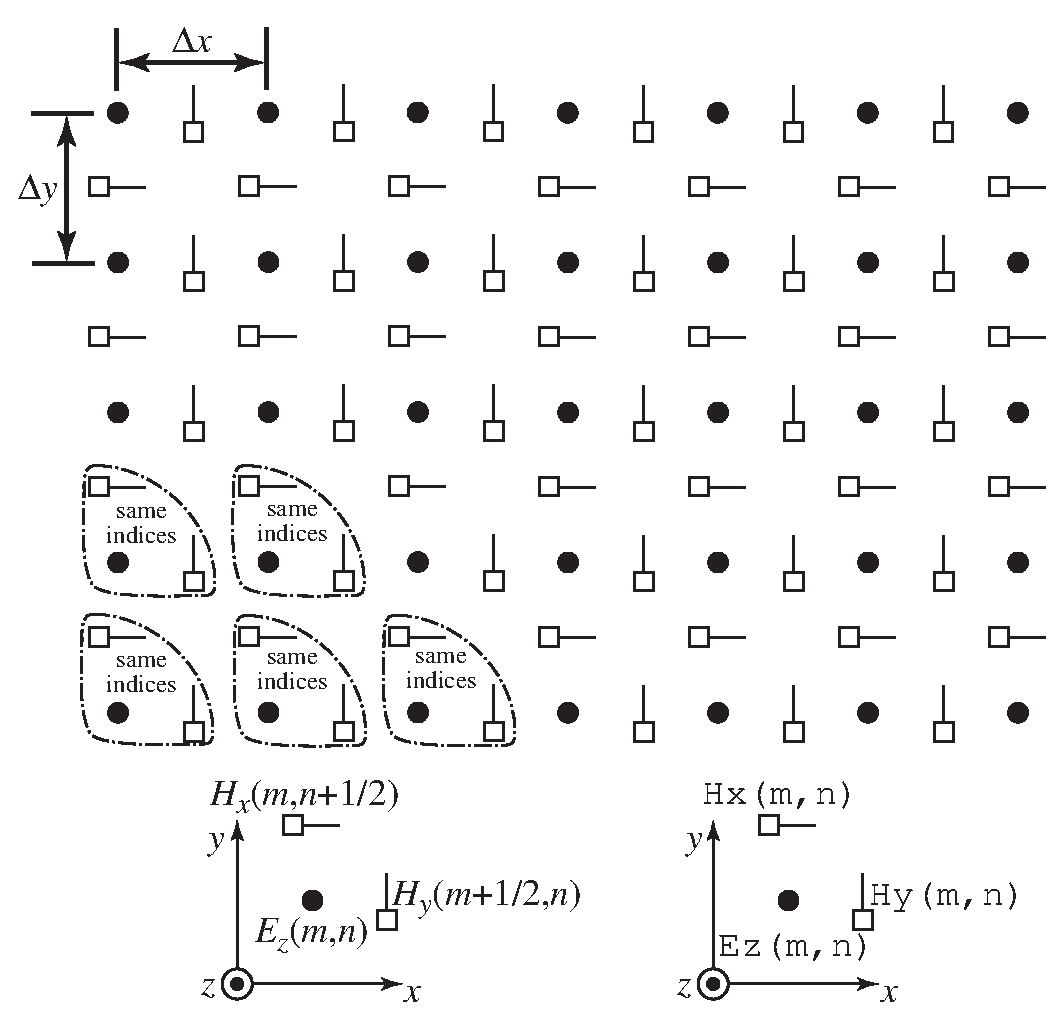
\epsfig{width=5in,file=Figures/Fdtd-multidimensional/tmz-fdtd-grid.eps}
\end{center} \caption{Spatial arrangement of electric- and
  magnetic-field nodes for TM$^z$ polarization.  The electric-field
  nodes are shown as circles and the magnetic-field nodes as squares
  with a line that indicates the orientation of the field component.
  The somewhat triangularly shaped dashed lines indicate groupings of
  nodes that have the same array indices.  For example, in the lower
  left corner of the grid all the nodes would have indices in a
  computer program of $(m=0,n=0)$.  In this case the spatial offset of
  the fields is implicitly understood.  This grouping is repeated
  throughout the grid.  However, groups at the top of the grid lack an
  $H_x$ node and groups at the right edge lack an $H_y$ node.  The
  diagram at the bottom left of the figure indicates nodes with their
  offsets given explicitly in the spatial arguments whereas the
  diagram at the bottom right indicates how the same nodes would be
  specified in a computer program where the offsets are understood
  implicitly.}  \label{fig:tmzGrid}
\end{figure}

When we say the dimensions of a TM$^z$ grid is $M\times N$, that
corresponds to the dimensions of the $E_z$ array.  We will ensure the
grid is terminated such that there are electric-field nodes on the
edge of the grid.  Thus, the $H_x$ array would by $M\times (N-1)$
while the $H_y$ array would be $(M-1)\times N$.

In the arrangement of nodes shown in Fig.\ \ref{fig:tmzGrid} we will
assume the electric field nodes fall at integer spatial steps and the
magnetic field nodes are offset a half spatial step in either the $x$
or $y$ direction.  As with one dimension, the electric field is
assumed to exist at integer multiples of the temporal step while both
magnetic fields components are offset a half time-step from the
electric fields.  With this arrangement in mind,
the finite difference approximation of \refeq{eq:faradayTMzX} expanded
about the space-time point $(m\Delx,(n+1/2)\Dely,q\Delt)$ is
\begin{eqnarray}
  \lefteqn{\hspace{-.4in}
    -\sigma_m \frac{\fdtdh{H_x}{m,n+\half}{q+\half} +
                 \fdtdh{H_x}{m,n+\half}{q-\half}}{2}
    -\mu\frac{\fdtdh{H_x}{m,n+\half}{q+\half} -
            \fdtdh{H_x}{m,n+\half}{q-\half}}{\Delt}
   =} \nonumber \\
  & &  \hspace{3.3in}
   \frac{\fdtd{E_z}{m,n+1}{q}-\fdtd{E_z}{m,n}{q}}{\Dely}.
  \label{eq:fdtdTMzX}
\end{eqnarray}
This can be solved for the future value
$\fdtdh{H_x}{m,n+\half}{q+\half}$ in terms of the ``past''
values.  The resulting update equation is
\begin{equation}
  \fdtdh{H_x}{m,n+\half}{q+\half} =
  \frac{1-\frac{\sigma_m\Delt}{2\mu}}{1+\frac{\sigma_m\Delt}{2\mu}}
  \fdtdh{H_x}{m,n+\half}{q-\half} -
  \frac{1}{1+\frac{\sigma_m\Delt}{2\mu}}
   \frac{\Delt}{\mu\Dely}\left(\fdtd{E_z}{m,n+1}{q}-
                               \fdtd{E_z}{m,n}{q}\right).
  \label{eq:updateHxTMz}
\end{equation}
As was the case in one dimension, the material parameters $\mu$ and
$\sigma_m$ are those which pertain at the given evaluation point.

The update equation for the $y$ component of the magnetic field is
obtained by the finite-difference approximation of
\refeq{eq:faradayTMzY} expanded about the space-time point
$((m+1/2)\Delx,n\Dely,q\Delt)$.  The resulting equation is 
\begin{equation}
  \fdtdh{H_y}{m+\half,n}{q+\half} =
  \frac{1-\frac{\sigma_m\Delt}{2\mu}}{1+\frac{\sigma_m\Delt}{2\mu}}
  \fdtdh{H_y}{m+\half,n}{q-\half} + 
  \frac{1}{1+\frac{\sigma_m\Delt}{2\mu}}
   \frac{\Delt}{\mu\Delx}\left(\fdtd{E_z}{m+1,n}{q}-
                               \fdtd{E_z}{m,n}{q}\right).
  \label{eq:updateHyTMz}
\end{equation}
Again, the material parameters $\mu$ and $\sigma_m$ are those which
pertain at the given evaluation point.  Note that $H_y$ nodes are
offset in space from $H_x$ nodes.  Hence the $\mu$ and $\sigma_m$
appearing in \refeq{eq:updateHxTMz} and \refeq{eq:updateHyTMz} are not
necessarily the same even when $m$ and $n$ are the same.

The electric-field update equation is obtained via the finite-difference
approximation of \refeq{eq:ampereTMzZ} expanded about
$(m\Delx,n\Dely,(q+1/2)\Delt)$:
\begin{eqnarray}
  \fdtd{E_z}{m,n}{q+1} &=&
  \frac{1-\frac{\sigma\Delt}{2\epsilon}}{1+\frac{\sigma\Delt}{2\epsilon}}
  \fdtd{E_z}{m,n}{q} + 
  \frac{1}{1+\frac{\sigma\Delt}{2\epsilon}}
  \left(
    \frac{\Delt}{\epsilon\Delx}
    \left\{
      \fdtdh{H_y}{m+\half,n}{q+\half} - \fdtdh{H_y}{m-\half,n}{q+\half}
    \right\}\right.
 \nonumber\\
  && \hspace{1.2in} \mbox{} - 
	\left.
    \frac{\Delt}{\epsilon\Dely}
    \left\{
      \fdtdh{H_x}{m,n+\half}{q+\half} - \fdtdh{H_x}{m,n-\half}{q+\half}
    \right\}
  \right).
\end{eqnarray}

A uniform grid is one in which the spatial step size is the same in
all directions.  Assuming a uniform grid such that
$\Delx=\Dely=\delta$, we define the following quantities
\begin{eqnarray}
\chxh(m,n+1/2) &=&
  \left.
    \frac{1-\frac{\sigma_m\Delt}{2\mu}}{1+\frac{\sigma_m\Delt}{2\mu}}
  \right|_{m\delta,(n+1/2)\delta}, \\
\chxe(m,n+1/2) &=&
  \left.
    \frac{1}{1+\frac{\sigma_m\Delt}{2\mu}}\frac{\Delt}{\mu\delta}
  \right|_{m\delta,(n+1/2)\delta}, \\
\chyh(m+1/2,n) &=&
  \left.
    \frac{1-\frac{\sigma_m\Delt}{2\mu}}{1+\frac{\sigma_m\Delt}{2\mu}}
  \right|_{(m+1/2)\delta,n\delta}, \\
\chye(m+1/2,n) &=&
  \left.
    \frac{1}{1+\frac{\sigma_m\Delt}{2\mu}}\frac{\Delt}{\mu\delta}
  \right|_{(m+1/2)\delta,n\delta}, \\
\ceze(m,n) &=& 
  \left.
  \frac{1-\frac{\sigma\Delt}{2\epsilon}}{1+\frac{\sigma\Delt}{2\epsilon}}
  \right|_{m\delta,n\delta}, \\
\cezh(m,n) &=& 
  \left.
  \frac{1}{1+\frac{\sigma\Delt}{2\epsilon}}
    \frac{\Delt}{\epsilon\delta}
  \right|_{m\delta,n\delta}.
\end{eqnarray}
These quantities appear in the update equations and employ the
following naming convention: the first letter identifies the quantity
as a constant which does not vary in time (one can also think of this
$C$ as representing the word coefficient), the next two letters
indicate the field being updated, and the last letter indicates the
type of field this quantity multiplies.  For example, $\chxh$
appears in the update equation for $H_x$ and it multiples the previous
value of the magnetic field.  On the other hand, $\chxe$, which
also appears in the update equation for $H_x$, multiplies the electric
fields.

To translate these update equations into a form that is suitable for
use in a computer program, we follow the approach that was used in
one dimension: explicit references to the time step are dropped and
the spatial offsets are understood.  As illustrated in Fig.\
\ref{fig:tmzGrid}, an $H_y$ node is assumed to be a half spatial step
further in the $x$ direction than the corresponding $E_z$ node with
the same indices.  Similarly, an $H_x$ node is assumed to be a half
spatial step further in the $y$ direction than the corresponding $E_z$
node with the same indices.  Thus, in C, the update equations could be
written
\begin{code}
  Hx(m, n) = Chxh(m, n) * Hx(m, n) - 
     Chxe(m, n) * (Ez(m, n + 1) - Ez(m, n));
  Hy(m, n) = Chyh(m, n) * Hy(m, n) + 
     Chye(m, n) * (Ez(m + 1, n) - Ez(m, n));
  Ez(m, n) = Ceze(m, n) * Ez(m, n) + 
     Cezh(m, n) * ((Hy(m, n) - Hy(m - 1, n)) - (Hx(m, n) - Hx(m, n - 1)));
\end{code}
The reason that the ``arrays'' appearing in these equations start with
an uppercase letter and use parentheses (instead of two pairs of
brackets that would be used with traditional two-dimensional arrays
in C) is because these terms are actually macros consistent with the
usage described in Sec.\ \ref{sec:multiArrays}.  In order for these
equations to be useful, they have to be contained within loops that
cycle over the spatial indices and these loops must themselves be
contained within a time-stepping loop.  Additional considerations are
initialization of the arrays, the introduction of energy, and
termination of the grid.  This issues are covered in the following sections.

\section{TM$^z$ Example}

To illustrate the simplicity of the FDTD method in two dimensions, let
us consider a simulation of a TM$^z$ grid which is $101$ nodes by $81$
nodes and filled with free space.  The grid will be terminated on
electric field nodes which will be left at zero (so that the
simulation is effectively of a rectangular resonator with PEC walls).
A Ricker wavelet with $20$ points per wavelength at its most energetic
frequency is hardwired to the electric-field node at the center of the
grid.  

Before we get to the core of the code, we are now at a point where it
is convenient to split the main header file into multiple header
files: one defining the {\tt Grid} structure, one defining various
macros, one giving the allocation macros, and one providing the
function prototypes.  Not all the ``{\tt .c}'' files need to include
each of these header files.

The arrangement of the code is shown in Fig.\ \ref{fig:filesTmZ}.  In
this figure the header files {\tt fdtd-grid1.h}, {\tt
fdtd-alloc1.h}, {\tt fdtd-macro-tmz.h}, and {\tt fdtd-proto1.h} are
shown in a single box but they exist as four separate files (as will
be shown below).

\begin{figure}
  \begin{center}
  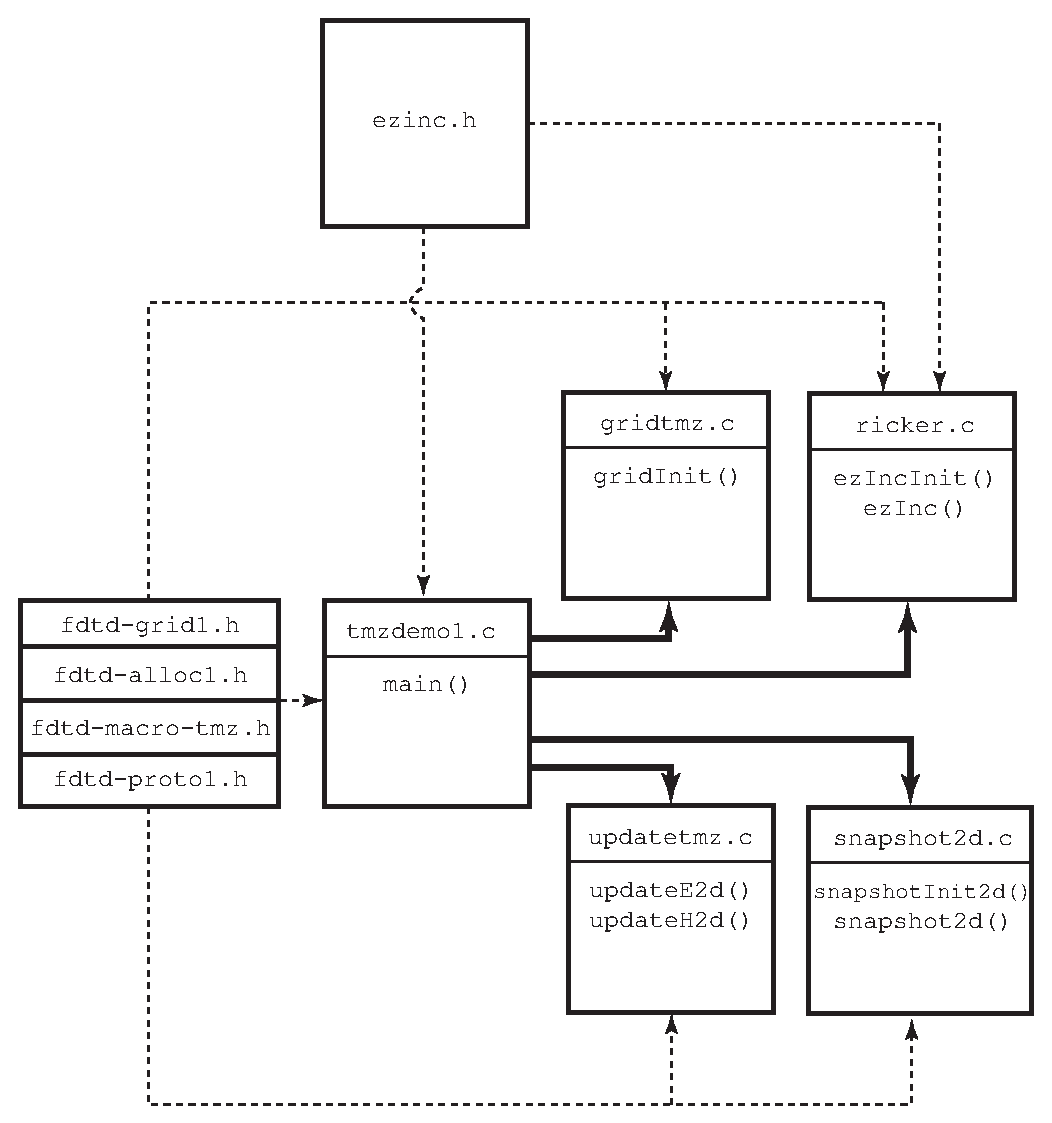
\epsfig{width=4.1in,file=Figures/Fdtd-multidimensional/tmzdemo1-files.eps}
  \end{center} \caption{The files associated with a simple TM$^z$
  simulation with a hard source at the center of the grid.  The four
  header files with an {\tt fdtd-} prefix are lumped into a single
  box.  Not all these files are included in each of the files to which
  this box is linked.  See the code for the specifics related to the
  inclusion of these files. }
  \label{fig:filesTmZ}
\end{figure}

The contents of {\tt fdtd-grid1.h} are shown in Program
\ref{pro:fdtdgrid1h}.  The {\tt Grid} structure, which begins on line
\ref{fdtdgrid1hB}, now has elements for any of the possible electric
or magnetic field components as well as their associated coefficient
arrays.  Note that just because all the pointers are declared, they do
not have to be used or point to anything useful.  The {\tt Grid}
structure shown here could be used for a 1D simulation---it provides
elements for everything that was needed to do a 1D simulation---but
most of the pointers would be unused, i.e., those elements that
pertain to anything other than a 1D simulation would be ignored.

The way we will distinguish between what different grids are being
used for is by setting the ``{\tt type}'' field of the grid.  Note
that line \ref{fdtdgrid1hA} creates a {\tt GRIDTYPE} enumeration.
This command merely serves to set the value of {\tt oneDGrid} to zero,
the value of {\tt teZGrid} to one, and the value of {\tt tmZGrid} to
two.  (The value of {\tt threeDGrid} would be three, but we are not
yet concerned with three-dimensional grids.)  A {\tt Grid} will have
its {\tt type} set to one of these values.  Functions can then check
the {\tt type} and act accordingly.

\begin{program}
{\tt fdtd-grid1.h}  Contents of the header file that defines the {\tt
Grid} structure.  This structure now contains pointers for each of the
possible field values.  However, not all these pointers would be used
for any particular grid.  The pointers that are meaningful would be
determined by the ``{\tt type}'' of the grid.  The {\tt type} takes on
one of the values of the {\tt GRIDTYPE} enumeration.
\label{pro:fdtdgrid1h}
\codemiddle
\begin{lstlisting}
#ifndef _FDTD_GRID1_H
#define _FDTD_GRID1_H

enum GRIDTYPE {oneDGrid, teZGrid, tmZGrid, threeDGrid}; /*@ \label{fdtdgrid1hA} @*/

struct Grid {                 /*@ \label{fdtdgrid1hB} @*/
  double *hx, *chxh, *chxe;
  double *hy, *chyh, *chye;
  double *hz, *chzh, *chze;
  double *ex, *cexe, *cexh;
  double *ey, *ceye, *ceyh;
  double *ez, *ceze, *cezh;
  int sizeX, sizeY, sizeZ;
  int time, maxTime;
  int type;
  double cdtds;
};

typedef struct Grid Grid;

#endif
\end{lstlisting}
\end{program}

The contents of {\tt fdtd-alloc1.h} are shown in Program
\ref{pro:fdtdalloc1h}.  This header file merely provides the
memory-allocation macros that have been discussed previously.

\begin{program}
{\tt fdtd-alloc1.h} Contents of the header file that defines the
memory allocation macros suitable for 1D and 2D arrays.
\label{pro:fdtdalloc1h}
\codemiddle
\begin{lstlisting}
#ifndef _FDTD_ALLOC1_H
#define _FDTD_ALLOC1_H

#include <stdio.h>
#include <stdlib.h>

/* memory allocation macros */
#define ALLOC_1D(PNTR, NUM, TYPE)                               \
    PNTR = (TYPE *)calloc(NUM, sizeof(TYPE));                   \
    if (!PNTR) {                                                \
      perror("ALLOC_1D");                                       \
      fprintf(stderr,                                           \
          "Allocation failed for " #PNTR ".  Terminating...\n");\
      exit(-1);                                                 \
    }

#define ALLOC_2D(PNTR, NUMX, NUMY, TYPE)                            \
    PNTR = (TYPE *)calloc((NUMX) * (NUMY), sizeof(TYPE));           \
    if (!PNTR) {                                                    \
      perror("ALLOC_2D");                                           \
      fprintf(stderr,                                               \
              "Allocation failed for " #PNTR ".  Terminating...\n");\
      exit(-1);                                                     \
    }

#endif
\end{lstlisting}
\end{program}

The contents of {\tt fdtd-macro-tmz.h} are shown in Program
\ref{pro:fdtdmacrotmzh}.  This file provides the macros used to access
the field arrays and elements of a pointer to a {\tt Grid} structure.
Thus far all the macros we have used assumed the {\tt Grid} pointer
was called {\tt g}.  The macros provided in lines
\ref{fdtdmacrotmzHA}--\ref{fdtdmacrotmzHB} no longer make this
assumption.  Instead, one specifies the name of the pointer as the
first argument.  To this point in our code there is no need for this
added degree of freedom.  We only considered code that has one pointer
to a {\tt Grid} and we have consistently named it {\tt g}.  However,
as we will see when we discuss the TFSF boundary, it is convenient to
have the ability to refer to different grids.

The macros in lines \ref{fdtdmacrotmzHC}--\ref{fdtdmacrotmzHD} do
assume the {\tt Grid} pointer is named {\tt g}.  These macros are
actually defined in terms of the first set of macros where the first
argument has been set to {\tt g}.  Note that although we are
discussing a 2D TM$^z$ problem, this file still provides macros that
can be used for a 1D array.  Again, we will see, when we implement a
2D TFSF boundary, that there are valid reasons for doing this.  Since
any function that is using these macros will also need to know about a
{\tt Grid} structure, line \ref{fdtdmacrotmzHE} ensures that the {\tt
  fdtd-grid1.h} header file is also included.

\begin{program}
{\tt fdtd-macro-tmz.h} Header file providing macros suitable for
accessing the elements and arrays of either a 1D or 2D {\tt Grid}.
There are two distinct sets of macros.  The first set takes an
argument that speficies the name of the pointer to the {\tt Grid}
structure.  The second set assumes the name of the pointer is {\tt g}.
\label{pro:fdtdmacrotmzh}
\codemiddle
\begin{lstlisting}
#ifndef _FDTD_MACRO_TMZ_H
#define _FDTD_MACRO_TMZ_H

#include "fdtd-grid1.h"    /*@ \label{fdtdmacrotmzHE} @*/

/* macros that permit the "Grid" to be specified */
/* one-dimensional grid */
#define Hy1G(G, M)      G->hy[M]   /*@ \label{fdtdmacrotmzHA} @*/
#define Chyh1G(G, M)    G->chyh[M]
#define Chye1G(G, M)    G->chye[M]

#define Ez1G(G, M)      G->ez[M]
#define Ceze1G(G, M)    G->ceze[M]
#define Cezh1G(G, M)    G->cezh[M]

/* TMz grid */
#define HxG(G, M, N)     G->hx[(M) * (SizeYG(G)-1) + (N)]
#define ChxhG(G, M, N) G->chxh[(M) * (SizeYG(G)-1) + (N)]
#define ChxeG(G, M, N) G->chxe[(M) * (SizeYG(G)-1) + (N)]

#define HyG(G, M, N)     G->hy[(M) * SizeYG(G) + (N)]
#define ChyhG(G, M, N) G->chyh[(M) * SizeYG(G) + (N)]
#define ChyeG(G, M, N) G->chye[(M) * SizeYG(G) + (N)]

#define EzG(G, M, N)     G->ez[(M) * SizeYG(G) + (N)]
#define CezeG(G, M, N) G->ceze[(M) * SizeYG(G) + (N)]
#define CezhG(G, M, N) G->cezh[(M) * SizeYG(G) + (N)]

#define SizeXG(G)        G->sizeX
#define SizeYG(G)        G->sizeY
#define SizeZG(G)        G->sizeZ
#define TimeG(G)         G->time
#define MaxTimeG(G)      G->maxTime
#define CdtdsG(G)        G->cdtds
#define TypeG(G)         G->type     /*@ \label{fdtdmacrotmzHB} @*/

/* macros that assume the "Grid" is "g" */
/* one-dimensional grid */
#define Hy1(M)      Hy1G(g, M)     /*@ \label{fdtdmacrotmzHC} @*/
#define Chyh1(M)    Chyh1G(g, M)
#define Chye1(M)    Chye1G(g, M)

#define Ez1(M)      Ez1G(g, M)
#define Ceze1(M)    Ceze1G(g, M)
#define Cezh1(M)    Cezh1G(g, M)

/* TMz grid */
#define Hx(M, N)   HxG(g, M, N)
#define Chxh(M, N) ChxhG(g, M, N)
#define Chxe(M, N) ChxeG(g, M, N) 

#define Hy(M, N)   HyG(g, M, N)
#define Chyh(M, N) ChyhG(g, M, N)
#define Chye(M, N) ChyeG(g, M, N)

#define Ez(M, N)   EzG(g, M, N)
#define Ceze(M, N) CezeG(g, M, N) 
#define Cezh(M, N) CezhG(g, M, N) 

#define SizeX        SizeXG(g)
#define SizeY        SizeYG(g)
#define SizeZ        SizeZG(g)
#define Time         TimeG(g)
#define MaxTime      MaxTimeG(g)
#define Cdtds        CdtdsG(g)
#define Type         TypeG(g)       /*@ \label{fdtdmacrotmzHD} @*/

#endif   /* matches #ifndef _FDTD_MACRO_TMZ_H */
\end{lstlisting}
\end{program}

Finally, the contents of {\tt fdtd-proto1.h} are shown in Program
\ref{pro:fdtdproto1}.  This file provides the prototypes for the
various functions associated with the simulation.  Since a pointer to
a {\tt Grid} appears as an argument to these functions, any file that
includes this header will also need to include {\tt fdtd-grid1.h} as
is done in line \ref{fdtdproto1A}.

\begin{program}
{\tt fdtd-proto1.h} Header file providing the function prototypes.
\label{pro:fdtdproto1}
\codemiddle
\begin{lstlisting}
#ifndef _FDTD_PROTO1_H
#define _FDTD_PROTO1_H

#include "fdtd-grid1.h"  /*@ \label{fdtdproto1A} @*/

/* Function prototypes */
void gridInit(Grid *g);

void snapshotInit2d(Grid *g);
void snapshot2d(Grid *g);

void updateE2d(Grid *g);
void updateH2d(Grid *g);

#endif
\end{lstlisting}
\end{program}

The file {\tt tmzdemo1.c}, which contains the {\tt main()} function,
is shown in Program \ref{pro:tmzdemo1}.  The program begins with the
inclusion of the necessary header files.  Note that only three of the
four {\tt fdtd-} header files are explicitly included.  However, both
the header files {\tt fdtd-macro-tmz.h} and {\tt fdtd-proto1.h} ensure
that the ``missing'' file, {\tt fdtd-grid1.h}, is included.

Fields are introduced into the grid by hardwiring the value of an
electric-field node as shown in line \ref{tmzdemo1A}.  Because the
source function is used in {\tt main()}, the header file {\tt ezinc.h}
had to be included in this file.  Other than those small changes, this
program looks similar to many of the 1D programs which we have
previously considered.

\begin{program}
{\tt tmzdemo1.c}
FDTD implementation of a TM$^z$ grid with a Ricker wavelet source at
the center of the grid.  No ABC have been implemented so the
simulation is effectively of a resonator.
\label{pro:tmzdemo1}
\codemiddle
\begin{lstlisting}
/* TMz simulation with Ricker source at center of grid. */

#include "fdtd-alloc1.h"
#include "fdtd-macro-tmz.h"
#include "fdtd-proto1.h"
#include "ezinc.h"

int main()
{
  Grid *g;

  ALLOC_1D(g, 1, Grid); // allocate memory for Grid

  gridInit(g);        // initialize the grid
  ezIncInit(g);
  snapshotInit2d(g);  // initialize snapshots

  /* do time stepping */
  for (Time = 0; Time < MaxTime; Time++) {
    updateH2d(g);     // update magnetic field
    updateE2d(g);     // update electric field
    Ez(SizeX / 2, SizeY / 2) = ezInc(Time, 0.0); // add a source /*@ \label{tmzdemo1A} @*/
    snapshot2d(g);    // take a snapshot (if appropriate)
  } // end of time-stepping

  return 0;
}
\end{lstlisting}
\end{program}

The contents of {\tt gridtmz.c}, which contains the grid
initialization function {\tt gridInit()}, is shown in Program
\ref{pro:gridtmz}.  On line \ref{gridtmzA} the type of grid is
defined.  This is followed by statements which set the size of the
grid, in both the $x$ and $y$ directions, the duration of the
simulation, and the Courant number.  Then, on lines \ref{gridtmzB}
through \ref{gridtmzC}, space is allocated for the field arrays and
their associated coefficients array.  Note that although the $E_z$
array is {\tt SizeX}$\times${\tt SizeY}, $H_x$ is {\tt
  SizeX}$\times(\mbox{\tt SizeY}-1)$, and $H_y$ is $(\mbox{\tt
  SizeX}-1)\times${\tt SizeY}.  The remainder of the program merely
sets the coefficient arrays.  Here there is no need to include the
header file {\tt fdtd-proto1.h} since this function does not call any
of the functions listed in that file.

\begin{program}
{\tt gridtmz.c} Grid initialization function for a TM$^z$ simulation.
Here the grid is simply homogeneous free space.
\label{pro:gridtmz}
\codemiddle
\begin{lstlisting}
#include "fdtd-macro-tmz.h"
#include "fdtd-alloc1.h"
#include <math.h>

void gridInit(Grid *g) {
  double imp0 = 377.0;
  int mm, nn;

  Type = tmZGrid;                          /*@ \label{gridtmzA} @*/
  SizeX = 101;             // x size of domain
  SizeY = 81;              // y size of domain
  MaxTime = 300;           // duration of simulation
  Cdtds = 1.0 / sqrt(2.0); // Courant number

  ALLOC_2D(g->hx,   SizeX, SizeY - 1, double);  /*@ \label{gridtmzB} @*/
  ALLOC_2D(g->chxh, SizeX, SizeY - 1, double);
  ALLOC_2D(g->chxe, SizeX, SizeY - 1, double);
  ALLOC_2D(g->hy,   SizeX - 1, SizeY, double);
  ALLOC_2D(g->chyh, SizeX - 1, SizeY, double);
  ALLOC_2D(g->chye, SizeX - 1, SizeY, double);
  ALLOC_2D(g->ez,   SizeX, SizeY, double);
  ALLOC_2D(g->ceze, SizeX, SizeY, double);
  ALLOC_2D(g->cezh, SizeX, SizeY, double);    /*@ \label{gridtmzC} @*/
 
  /* set electric-field update coefficients */
  for (mm = 0; mm < SizeX; mm++)
    for (nn = 0; nn < SizeY; nn++) {
      Ceze(mm, nn) = 1.0;
      Cezh(mm, nn) = Cdtds * imp0;
    }

  /* set magnetic-field update coefficients */
  for (mm = 0; mm < SizeX; mm++)
    for (nn = 0; nn < SizeY - 1; nn++) {
      Chxh(mm, nn) = 1.0;
      Chxe(mm, nn) = Cdtds / imp0;
    }

  for (mm = 0; mm < SizeX - 1; mm++)
    for (nn = 0; nn < SizeY; nn++) {
      Chyh(mm, nn) = 1.0;
      Chye(mm, nn) = Cdtds / imp0;
    }

  return;
}
\end{lstlisting}
\end{program}

The functions for updating the fields are contained in the file {\tt
  updatetmz.c} which is shown in Program \ref{pro:updatetmz}.  In line
\ref{updatetmzA} the {\tt Type} is checked (i.e., {\tt g->type} is
checked).  If it is {\tt oneDGrid} then only the $H_y$ field is
updated and it only has a single spatial index.  If the grid is not a
1D grid, it is assumed to be a TM$^z$ grid.  Thus, starting on line
\ref{updatetmzB}, $H_x$ and $H_y$ are updated and they now have two
spatial indices.

\begin{program}
{\tt updatetmz.c} Functions to update the fields.  Depending on the
type of grid, the fields can be treated as either one- or
two-dimensional.  
\label{pro:updatetmz}
\codemiddle
\begin{lstlisting}
#include "fdtd-macro-tmz.h"

/* update magnetic field */
void updateH2d(Grid *g) {
  int mm, nn;

  if (Type == oneDGrid) {  /*@ \label{updatetmzA} @*/
    for (mm = 0; mm < SizeX - 1; mm++)
      Hy1(mm) = Chyh1(mm) * Hy1(mm) 
	+ Chye1(mm) * (Ez1(mm + 1) - Ez1(mm));
  } else { 
    for (mm = 0; mm < SizeX; mm++) /*@ \label{updatetmzB} @*/
      for (nn = 0; nn < SizeY - 1; nn++)
	Hx(mm, nn) = Chxh(mm, nn) * Hx(mm, nn) 
	  - Chxe(mm, nn) * (Ez(mm, nn + 1) - Ez(mm, nn));

    for (mm = 0; mm < SizeX - 1; mm++)
      for (nn = 0; nn < SizeY; nn++)
	Hy(mm, nn) = Chyh(mm, nn) * Hy(mm, nn) 
	  + Chye(mm, nn) * (Ez(mm + 1, nn) - Ez(mm, nn));
  }

  return;
}

/* update electric field */
void updateE2d(Grid *g) {
  int mm, nn;

  if (Type == oneDGrid) {  /*@ \label{updatetmzC} @*/
    for (mm = 1; mm < SizeX - 1; mm++)
      Ez1(mm) = Ceze1(mm) * Ez1(mm) 
	+ Cezh1(mm) * (Hy1(mm) - Hy1(mm - 1));
  } else { 
    for (mm = 1; mm < SizeX - 1; mm++)
      for (nn = 1; nn < SizeY - 1; nn++)
	Ez(mm, nn) = Ceze(mm, nn) * Ez(mm, nn) +
	  Cezh(mm, nn) * ((Hy(mm, nn) - Hy(mm - 1, nn)) -
		       (Hx(mm, nn) - Hx(mm, nn - 1)));
  }

  return;
}
\end{lstlisting}
\end{program}

The function for updating the electric field, {\tt updateE2d()}, only
is responsible for updating the $E_z$ field.  However, as shown in
line \ref{updatetmzC}, it still must check the grid type.  If this is
a 1D grid, $E_z$ only has a single spatial index and only depends on
$H_y$.  If it is not a 1D grid, it is assumed to be a TM$^z$ grid and
$E_z$ now depends on both $H_x$ and $H_y$.

The function to implement the Ricker wavelet is shown in Program
\ref{pro:ricker}.  The header file {\tt ezinc.h} is virtually
unchanged from Program \ref{pro:ezincH}.  The one minor change is that
instead of including {\tt fdtd2.h}, now the file {\tt
  fdtd-macro-tmz.h} is included.  Thus {\tt ezinc.h} is not shown.
The initialization function {\tt ezIncInit()} prompts the user to
enter the points per wavelength at which the Ricker wavelet has
maximum energy.  In line \ref{ezinc2DA} it also makes a local copy of
the Courant number (since the {\tt Grid} is not passed to the {\tt
  ezInc()} function and would not otherwise know this value).

\begin{program}
{\tt ricker.c} 
Function to implement a Ricker wavelet.  This is a traveling-wave
version of the function so {\tt ezInc()} takes arguments of both time
and space.
\label{pro:ricker}
\codemiddle
\begin{lstlisting}
#include "ezinc.h"

static double cdtds, ppw = 0;

/* initialize source-function variables */
void ezIncInit(Grid *g){

  printf("Enter the points per wavelength for Ricker source: ");
  scanf(" %lf", &ppw);
  cdtds = Cdtds;   /*@ \label{ezinc2DA} @*/
  return;
}

/* calculate source function at given time and location */
double ezInc(double time, double location) {
  double arg;

  if (ppw <= 0) {
    fprintf(stderr,
       "ezInc: ezIncInit() must be called before ezInc.\n"
       "       Points per wavelength must be positive.\n");
    exit(-1);
  }

  arg = M_PI * ((cdtds * time - location) / ppw - 1.0);
  arg = arg * arg;

  return (1.0 - 2.0 * arg) * exp(-arg);
}
\end{lstlisting}
\end{program}

Finally, {\tt snapshot2d.c} is shown in Program \ref{pro:snap2d}.  The
function {\tt snapshotInit2d()} obtains information from the user
about the output that is desired.  The goal is to write the data so
that the electric field can be visualized over the entire 2D
computational domain.

\begin{program}
{\tt snapshot2d.c} Function to record the 2D field to a file.  The
data is stored as binary data. 
\label{pro:snap2d}
\codemiddle
\begin{lstlisting}
#include <stdio.h>
#include <stdlib.h>
#include "fdtd-macro-tmz.h"

static int temporalStride = -2, frame = 0, startTime,
  startNodeX, endNodeX, spatialStrideX,
  startNodeY, endNodeY, spatialStrideY;
static char basename[80];

void snapshotInit2d(Grid *g) {
  
  int choice;
  
  printf("Do you want 2D snapshots? (1=yes, 0=no) ");
  scanf("%d", &choice);
  if (choice == 0) {
    temporalStride = -1;
    return;
  }

  printf("Duration of simulation is %d steps.\n", MaxTime);
  printf("Enter start time and temporal stride: ");
  scanf(" %d %d", &startTime, &temporalStride);
  printf("In x direction grid has %d total nodes"
        " (ranging from 0 to %d).\n", SizeX, SizeX - 1);
  printf("Enter first node, last node, and spatial stride: ");
  scanf(" %d %d %d", &startNodeX, &endNodeX, &spatialStrideX);
  printf("In y direction grid has %d total nodes"
        " (ranging from 0 to %d).\n", SizeY, SizeY - 1);
  printf("Enter first node, last node, and spatial stride: ");
  scanf(" %d %d %d", &startNodeY, &endNodeY, &spatialStrideY);
  printf("Enter the base name: ");
  scanf(" %s", basename);

  return;
}

void snapshot2d(Grid *g) {
  int mm, nn;
  float dim1, dim2, temp;
  char filename[100];
  FILE *out;

  /* ensure temporal stride set to a reasonable value */
  if (temporalStride == -1) {
    return;
  } if (temporalStride < -1) {
    fprintf(stderr,
      "snapshot2d: snapshotInit2d must be called before snapshot.\n"
      "            Temporal stride must be set to positive value.\n");
    exit(-1);
  }

  /* get snapshot if temporal conditions met */
  if (Time >= startTime && 
      (Time - startTime) % temporalStride == 0) {
    sprintf(filename, "%s.%d", basename, frame++);
    out = fopen(filename, "wb");  /*@ \label{snap2dA} @*/

    /* write dimensions to output file -- 
     * express dimensions as floats */
    dim1 = (endNodeX - startNodeX) / spatialStrideX + 1;
    dim2 = (endNodeY - startNodeY) / spatialStrideY + 1;
    fwrite(&dim1, sizeof(float), 1, out);  /*@ \label{snap2dB} @*/
    fwrite(&dim2, sizeof(float), 1, out);  /*@ \label{snap2dC} @*/

    /* write remaining data */
    for (nn = endNodeY; nn >= startNodeY; nn -= spatialStrideY)   /*@ \label{snap2dD} @*/
      for (mm = startNodeX; mm <= endNodeX; mm += spatialStrideX) {
	temp = (float)Ez(mm, nn); // store data as a float   /*@ \label{snap2dE} @*/
	fwrite(&temp, sizeof(float), 1, out); // write the float
      }

    fclose(out);  // close file
  }

  return;
}
\end{lstlisting}
\end{program}

Similar to the snapshot code in one dimension, the $E_z$ field is
merely recorded (in binary format) to a file at the appropriate
time-steps.  It is up to some other program or software to render this
data in a suitable way.  In order to understand what is happening in
the two-dimensional grid, it is extremely helpful to display the
fields in a manner that is consistent with the underlying
two-dimensional format.  This can potentially be quite a bit of data.
To deal with it efficiently, it is often best to store the data
directly in binary format, which we will refer to as ``raw'' data.  In
line \ref{snap2dA} the output file is opened as a binary file (hence
``{\tt b}'' which appears in the second argument of the call to {\tt
fopen()}).

The arrays being used to store the fields are doubles.  However,
storing a complete double can be considered overkill when it comes to
generating graphics.  We certainly do not need $15$ digits of
precision when viewing the fields.  Instead of writing doubles, the
output is converted to a float. (By using floats instead of doubles,
the file size is reduced by a factor of two.)  Within each output data
file, first the dimensions of the array are written, as floats, as
shown in lines \ref{snap2dB} and \ref{snap2dC}.  After that, starting
in line \ref{snap2dD} of Program \ref{pro:snap2d}, two nested loops
are used to write each element of the array.  Note that the elements
are not written in what might be considered a standard way.  The
elements are written consistent with how you would read a book in
English: from left to right, top to bottom.  As mentioned previously,
this is not the most efficient way to access arrays, but there are
some image-processing tools which prefer that data be stored this way.

Once this data is generated, there are several ways in which the data
can be displayed.  It is possible to read the data directly using
Matlab and even create an animation of the field.  Appendix
\ref{ap:render2d} presents a Matlab function that can be used to
generate a movie from the data generated by Program \ref{pro:tmzdemo1}.

After compiling Program \ref{pro:tmzdemo1} in accordance with all the
files shown in Fig.\ \ref{fig:filesTmZ}, let us assume the executable
is named {\tt tmzdemo1}.  The following shows a typical session where
this program is run on a UNIX system (where the executable is entered
at the command-line prompt of ``{\tt >}'').  The user's entries are
shown in bold.
\begin{lstlisting}[numbers=none]
> /*b*/tmzdemo1/*n*/
Enter the points per wavelength for Ricker source: /*b*/20/*n*/
Do you want 2D snapshots? (1=yes, 0=no) /*b*/1/*n*/
Duration of simulation is 300 steps.
Enter start time and temporal stride: /*b*/10 10/*n*/
In x direction grid has 101 total nodes (ranging from 0 to 100).
Enter first node, last node, and spatial stride: /*b*/0 100 1/*n*/
In y direction grid has 81 total nodes (ranging from 0 to 80).
Enter first node, last node, and spatial stride: /*b*/0 80 1/*n*/
Enter the base name: /*b*/sim/*n*/
\end{lstlisting}
In this case the user set the Ricker wavelet to have $20$ points per
wavelength at the most energetic frequency.  Snapshots were generated
every $10$ time-steps beginning at the $10$th time-step.  The
snapshots were taken of the entire computational domain since the
start- and stop-points were the first and last nodes in the $x$ and
$y$ directions and the spatial stride was unity.  The snapshots had a
common base name of {\tt sim}.

Figure \ref{fig:tmzSnapshots} shows three snapshots of the electric
field that are generated by Program \ref{pro:tmzdemo1}.  These images
are individual frames generated by the code presented in Appendix
\ref{ap:render2d} (the frames are in color when viewed on a suitable
output device).  These frames correspond to snapshots taken at
time-steps $30$, $70$, and $110$.  Logarithmic scaling is used so that
the maximum normalized value of one corresponds to the color
identified as zero on the color-bar to the right of each image.  A
normalization value of unity was used for these images.  Three decades
are displayed so that the minimum visible normalized field is
$10^{-3}$.  This value is shown with a color corresponding to $-3$ on
the color-bar (any values less than the minimum are also displayed
using this same color).

\begin{figure}
  \begin{center}
  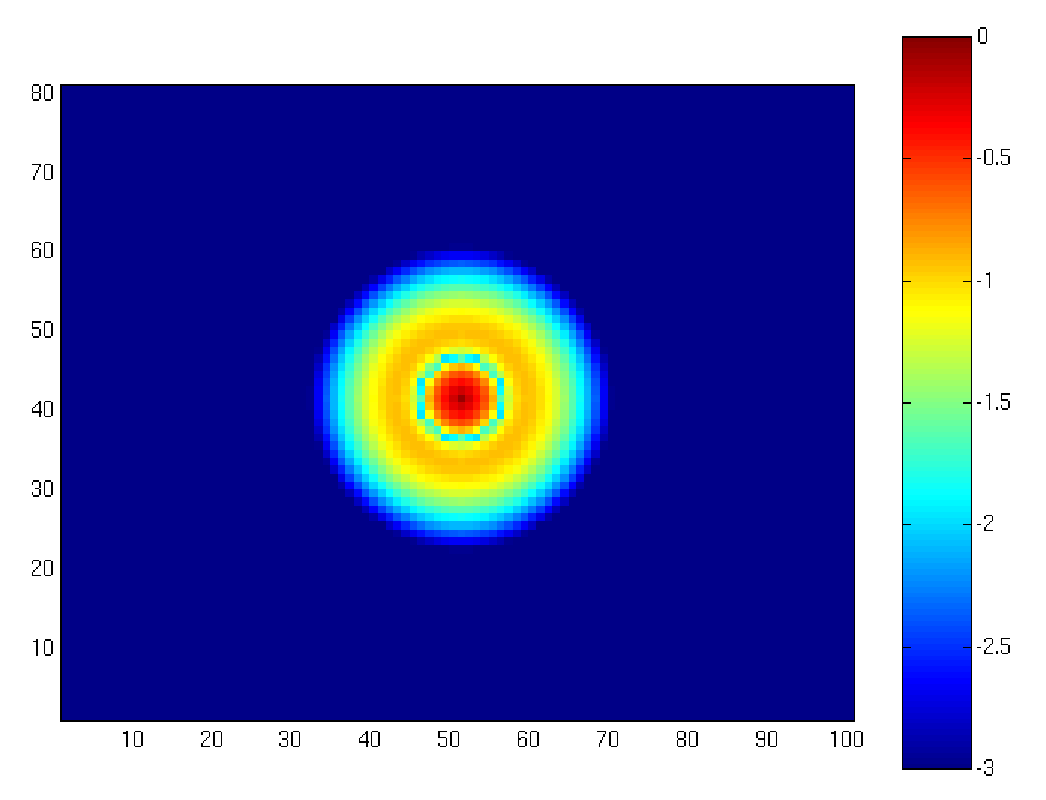
\epsfig{width=3in,file=Code/Fdtd-multidimensional/snapshot-sim3.eps}
  \\ (a) \\
  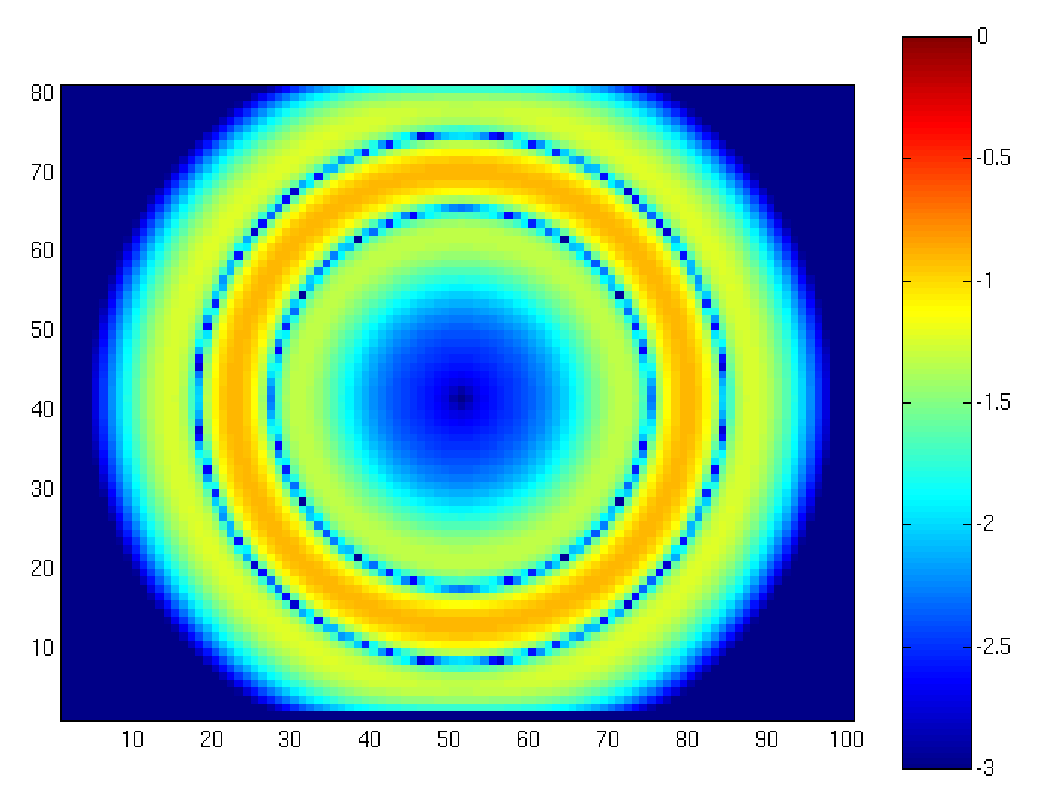
\epsfig{width=3in,file=Code/Fdtd-multidimensional/snapshot-sim7.eps}
  \\ (b) \\
  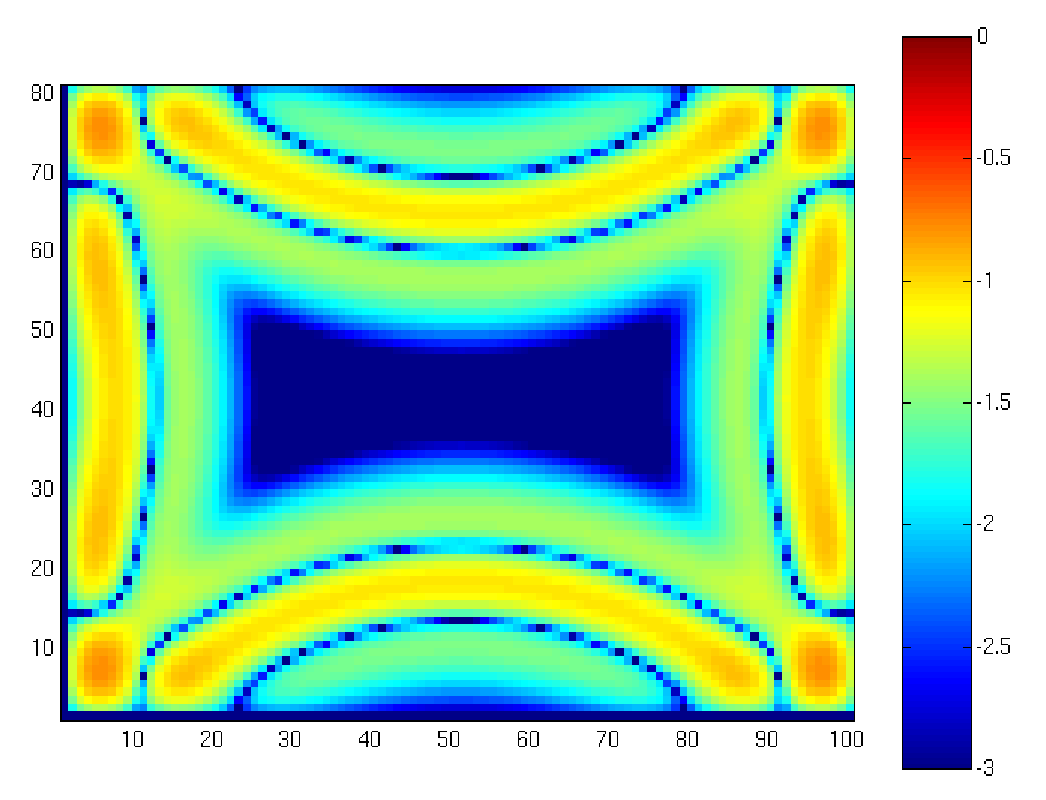
\epsfig{width=3in,file=Code/Fdtd-multidimensional/snapshot-sim11.eps}
  \\ (c) \end{center} \caption{Display of $E_z$ field generated by
  Program\ \ref{pro:tmzdemo1} at time steps (a) $30$, (b) $70$, and
  (c) $110$.  A Ricker source with $20$ points per wavelength at its
  most energetic frequency is hard-wired to the $E_z$ node at the
  center of the grid.}  \label{fig:tmzSnapshots}
\end{figure}

At time-step $30$, the field is seen to be radiating concentrically
away from the source at the center of the grid.  At time-step $70$ the
field is just starting to reach the top and bottom edges of the
computational domain.  Since the electric-field nodes along the edge
of the computational domain are not updated (due to these nodes
lacking a neighboring magnetic-field node in their update equations),
these edges behave as PEC boundaries.  Hence the field is reflected
back from these walls.  The reflection of the field in clearly
evident at time-step $110$.  As the simulation progresses, the field
bounces back and forth.  (The field at a given point can be recorded
and then Fourier transformed.  The peaks in the transform correspond
to the resonant modes of this particular structure.)

To model an infinite domain, the second-order ABC discussed in Sec.\
\ref{sec:secondOrderABC} can be applied to every electric field node
on the boundary.  In one dimension the ABC needed to be applied to
only two nodes.  In two dimensions, there would essentially be four
lines of nodes to which the ABC must be applied: nodes along the left,
right, top, and bottom.  However, in all cases the form of the ABC is
the same.  For a second-order ABC, a node on the boundary depends on
two interior nodes as well as the field at the boundary and those same
two interior nodes at two previous time steps.  As before, the old
values would have to be stored in supplementary arrays---six old
values for each node on the boundary.  This is accomplished fairly
easily by extrapolating the 1D case so that there are now four storage
arrays (one for the left, right, top, and bottom).  These would be
three-dimensional arrays.  In addition to two indices which indicate
displacement from the edge (i.e., displacement into the interior) and
the time step, there would be a third index to indicate displacement
{\em along} the edge.  So, for example, this third index would specify
the particular node along the top or bottom (and hence would vary
between $0$ and ``{\tt SizeX - 1}'') or the node along the left or right
(and hence would vary between $0$ and ``{\tt SizeY - 1}'').

For nodes in the corner of the computational domain, there is some
ambiguity as to which nodes are the neighboring ``interior'' nodes
which should be used by the ABC.  However, the corner nodes never
couple back to the interior and hence it does not matter what one does
with these nodes.  They can be left zero or assumed to contain
meaningless numbers and that will not affect the values in the
interior of the grid.  The magnetic fields that are adjacent to corner
nodes are affected by the values of the field in the corners.
However, these nodes themselves are not used be any other nodes in
their updates.  The electric fields which are adjacent to these
magnetic fields are updated using the ABC; they ignore the field at
the neighboring magnetic-field nodes.  Therefore no special
consideration will be given to resolving the corner ambiguity.


%%%%%%%%%%%%%%%%%%%%%%%%%%%%%%%%%%%%%%%%%%%%%%%%%%%%%%%%%%%%%%%%%%%%%%%%%%%
\section{The TFSF Boundary for TM$^z$ Polarization}

For a distant source illuminating a scatterer, it is not feasible to
discretize the space surrounding the source, discretize the space
between the source and the scatterer, and discretize the space
surrounding the scatterer.  Even if a large enough computer could be
obtained that was capable of storing all that discretized space, one
simply would not want to use the FDTD grid to propagate the field from
the source to the scatterer.  Such an endeavor would be slow,
incredibly inefficient, and suffer from needless numerical artifacts.
Instead, one should discretize the space surrounding the scatterer and
introduce the incident field via a total-field/scattered-field
boundary.  When the source is distant from the scatterer, the incident
field is nearly planar and thus we will restrict consideration to
incident plane waves.

Section \ref{sec:tfsf} showed how the TFSF concept could be
implemented in a one-dimensional problem.  The TFSF boundary separated
the grid into two regions: a total-field (TF) region and a
scattered-field (SF) region.  There were two nodes adjacent to this
boundary.  One was in the SF region and depended on a node in the TF
region.  The other was in the TF region and depended on a node in the
SF region.  To obtain self-consistent update equations, when updating
nodes in the TF region, one must use the total field which pertains at
the neighboring nodes.  Conversely, when updating nodes in the SF
region, one must use the scattered field which pertains at neighboring
nodes.  In one dimension, the two nodes adjacent to the boundary must
have the incident field either added to or subtracted from the field
which exists at their neighbor on the other side of the boundary.
Thus, in one dimension we required knowledge of the incident field at
two locations for every time step.

In two dimensions, the grid is again divided into a TF region and a SF
region.  In this case the boundary between the two regions is no
longer a point.  Figure \ref{fig:tmzTfsf} shows a TM$^z$ grid with a
rectangular TFSF boundary.  (The boundary does not have to be
rectangular, but the implementation details are simplest when the
boundary has straight sides and hence we will restrict ourselves to
TFSF boundaries which are rectangular.)  In this figure the TF region
is enclosed within the TFSF boundary which is drawn with a dashed
line.  The SF region is any portion of the grid that is outside this
boundary.  Nodes that have a neighbor on the other side of the
boundary are enclosed in a solid rectangle with rounded corners.  Note
that these encircled nodes are tangential to the TFSF boundary (we
consider the $E_z$ field, which points out of the page, to be
tangential to the boundary if we envision the boundary extending into
the third dimension).  The fields that are normal to the boundary,
such as the $H_y$ nodes along the top and bottom of the TFSF boundary,
do not have neighbors which are across the boundary (even though the
field could be considered adjacent to the boundary).  
\begin{figure}
  \begin{center}
  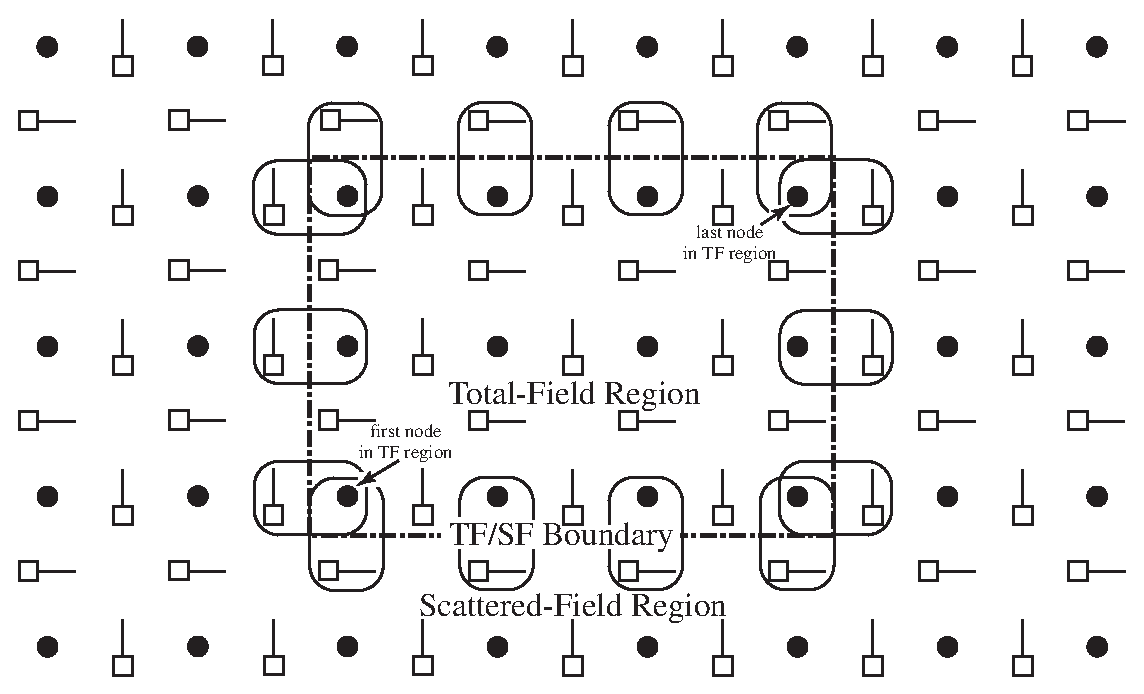
\epsfig{width=5.5in,file=Figures/Fdtd-multidimensional/tmz-fdtd-tfsf.eps}
  \end{center} \caption{Depiction of a total-field/scattered-field
  boundary in a TM$^z$ grid.  The size of the TF region is defined by
  the indices of the first and last electric field nodes which are
  within the region.  Note that at the right-hand side of the boundary
  the $H_y$ nodes with the same $x$-index (i.e., the same ``$m$''
  index) as the ``last'' node will be in the SF region.  Similarly, at
  the top of the grid, $H_x$ nodes with the same $y$-index as the last
  node will be in the SF region.  Therefore one must pay attention to
  the field component as well as the indices to determine if a node is
  in the SF or TF region.} \label{fig:tmzTfsf}
\end{figure}

In the implementation used here, the TF region is defined by the
indices of the ``first'' and ``last'' electric-field nodes which are
in the TF region.  These nodes are shown in Fig.\ \ref{fig:tmzTfsf}
where the ``first'' node is the one in the lower left corner and the
``last'' one is in the upper right corner.  Note that electric fields
and magnetic fields with the same indices are not necessarily on the
same side of the boundary.  For example, the $E_z$ nodes on the right
side of the TF region have one of their neighboring $H_y$ nodes in the
SF region.  This is true despite the fact that these $H_y$ nodes share
the same $x$-index as the $E_z$ nodes.

Further note that in this particular construction of a TFSF boundary,
the electric fields tantential to the TFSF boundary are always in the
TF region.  These nodes will have at least one neighboring magnetic
field node that is in the SF region.  Thus, the correction necessary
to obtain a consistent update of these electric field nodes would
involve adding the incident field the neighboring magnetic fields on
the other side of the TFSF boundary.  Conversely, the magnetic field
nodes that are tangential to the TFSF boundary are always in the SF
region.  These nodes will have one neighboring electric field node
that is in the TF region.  Thus, the correction necessary to obtain a
consistent update of these magnetic field nodes would involve
subtracting the incident field from the electric field node on the
other side of the TFSF boundary.

As in the one-dimensional case, to implement the TFSF method, one must
know the incident field at every node which has a neighbor on the
other side of the TFSF boundary.  The incident field must be known at
all these points and for every time-step.  In Section \ref{sec:tfsf}
analytic expressions were used for the incident field, i.e., the
expressions that describes propagation of the incident field in the
continuous world.  However, the incident field does not propagate the
same way in the FDTD grid as the continuous world (except in the
special case of one-dimensional propagation with a Courant number of
unity).  Therefore, if the continuous-world expressions were used for
the incident field, there would be a mismatch between the fields in
the grid and the fields given by the continuous-world expressions.
This mismatch would cause fields to leak across the boundary.  Another
drawback to using the continuous-world expressions is that they
typically involve a transcendental function (such as a trigonometric
function or an exponential).  Calculation of these functions is
somewhat computationally expensive---at least compared to a few simple
algebraic calculations.  If the transcendental functions have to be
calculated at numerous points for every time-step, this can impose a
potentially significant computational cost.  Fortunately, provided the
direction of the incident-field propagation coincides with one of the
axes of the grid, there is a way to ensure that the incident field
exactly matches the way in which the incident field propagates in the
two-dimensional FDTD grid.  Additionally, the calculation of the
incident field can be done efficiently.

The trick to calculating the incident field is to perform an auxiliary
one-dimensional FDTD simulation which calculates the incident field.
This auxiliary simulation uses the same Courant number and material
parameters as pertain in the two-dimensional grid but is otherwise
completely separate from the two-dimensional grid.  The
one-dimensional grid is merely used to find the incident fields needed
to implement the TFSF boundary.  (Each $E_z$ and $H_y$ node in the 1D
grid can be thought as providing $E_z^{\mathrm{inc}}$ and
$H_y^{\mathrm{inc}}$, respectively, at the appropriate point in
space-time as dictated by the discretization and time-stepping.)

Figure \ref{fig:tmzTfsfWith1D} shows the auxiliary 1D grid together
with the 2D grid.
\begin{figure}
  \begin{center}
  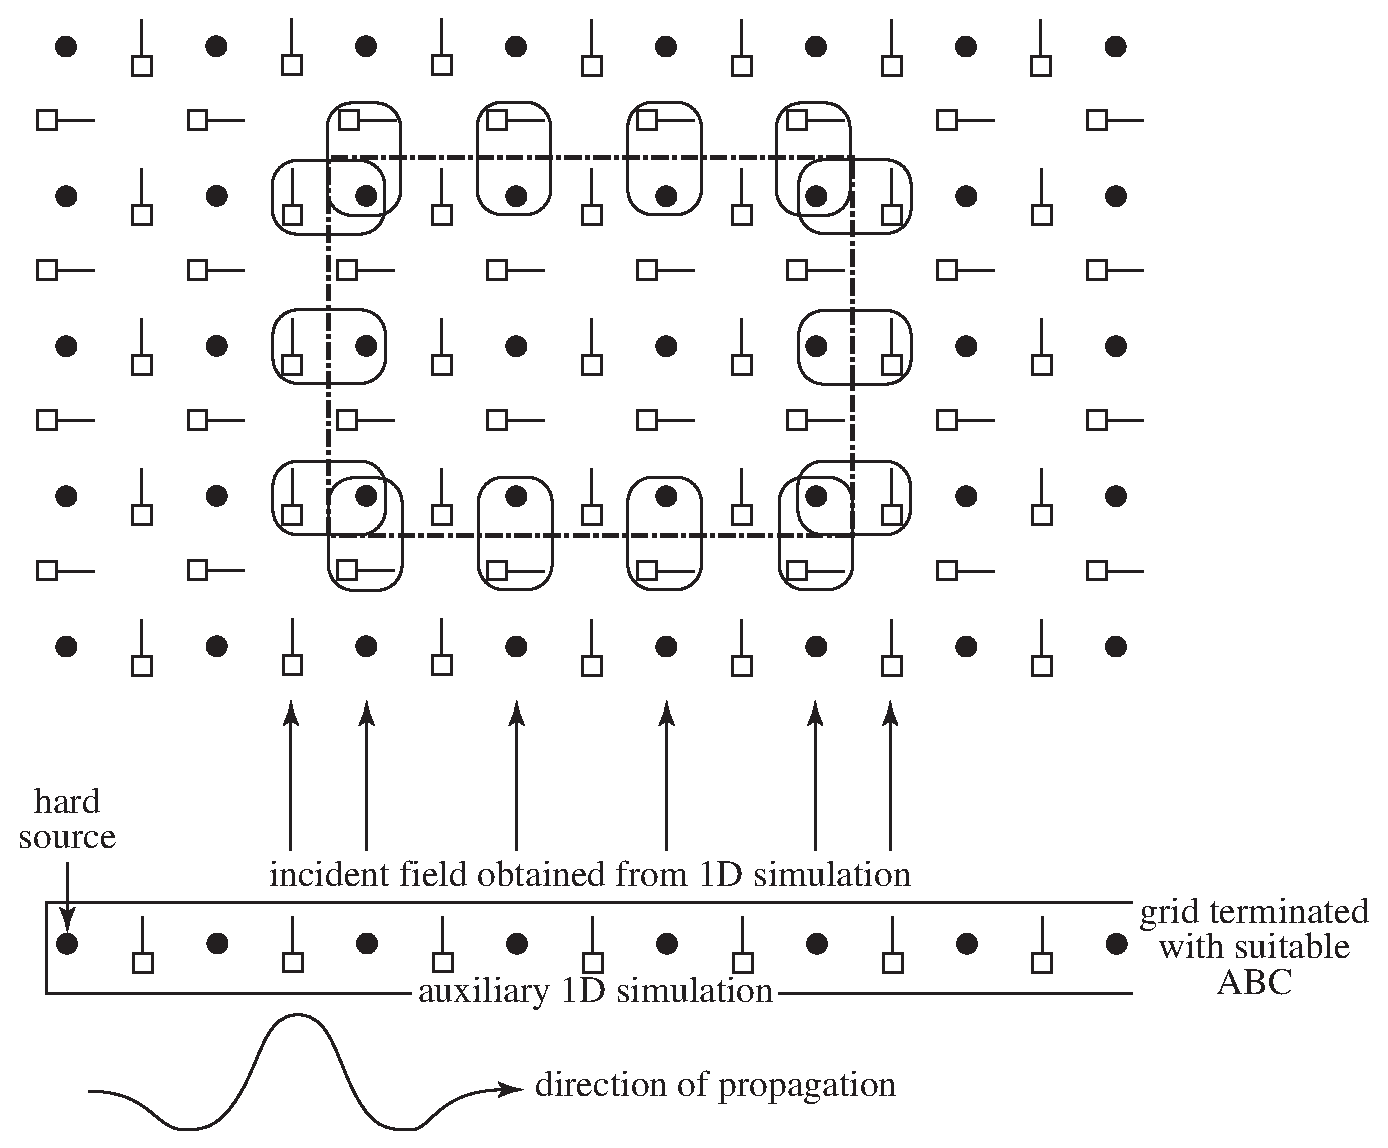
\epsfig{width=5.5in,file=Figures/Fdtd-multidimensional/tmz-fdtd-tfsf-with-1d.eps}
  \end{center} 
  \caption{A one-dimensional auxiliary grid is used to calculate the
  incident field which is assumed to be propagating in the $+x$
  direction.  The vertical arrows indicate the nodes whose values are
  needed to implement the TFSF boundary.  The incident $H_x$ field is
  zero and hence no correction is needed in association with $E_z$
  nodes that have a neighboring $H_x$ node on the other side of the
  boundary.  The 1D 
  grid is driven by a hard source at the left side.  The 1D grid must
  be suitably terminated at the right side to model an infinite domain.
  The size of the 1D grid is somewhat independent of the size of the
  2D grid---it must be large enough to provide incident field
  associated with each of the vertical arrows shown above but
  otherwise may be larger or smaller than the overall width of the 2D grid.
  \label{fig:tmzTfsfWith1D}}
\end{figure}
The base of the vertical arrows pointing from the 1D grid to the 2D
grid indicate the nodes in the 1D grid from which the nodes in the 2D
grid obtain the incident field (only nodes in the 2D grid adjacent to
the TFSF boundary require knowledge of the incident field).  Since the
incident field propagates in the $+x$ direction, there is no incident
$H_x$ field.  Hence nodes that depend on an $H_x$ node on the other
side of the TFSF boundary do not need to be corrected since
$H_x^{\mathrm{inc}}=0$.  

Despite the representation in Fig.\ \ref{fig:tmzTfsfWith1D}, the 1D
grid does not need to be the same width as the 2D grid, but it must be
at least as long as necessary to provide the incident field for all
the nodes tangential to the TFSF boundary (i.e., it must be large
enough to provide the values associated with the base of each of the
vertical arrows shown in Fig.\ \ref{fig:tmzTfsfWith1D}).
Additionally, the 1D grid must include a source on the left and the
right side of the grid must be suitably terminated so that the
incident field does not reflect back.  Here we will assume fields are
introduced into the 1D grid via a hard source at the left end.

Using an auxiliary 1D grid, the TFSF boundary could be realized as
follows.  First, outside of the time-stepping loop, a function would
be called to initialize the TFSF code.  This initialization would
allocate arrays of the necessary size for the 1D auxiliary grid and
set all the necessary constants.  Then, within
the time-stepping loop, the following steps would be taken (where we
use the additional subscripts $1\mathrm{D}$ and $2\mathrm{D}$ to
distinguish between arrays associated with the 1D and 2D grids):
\begin{enumerate}
\label{page:tfsfUpdateAlgorithm}
\item Update the magnetic fields in the two-dimensional grid using the
  usual update equations (i.e., do not account for the existence of
  TFSF boundary): $H_{x2\mathrm{D}}^{q-\half} \Rightarrow
  H_{x2\mathrm{D}}^{q+\half}$ and $H_{y2\mathrm{D}}^{q-\half}
  \Rightarrow H_{y2\mathrm{D}}^{q+\half}$.
\item Call a function to make all calculations and corrections
  associated with the TFSF boundary:
\begin{enumerate}
\item Correct the two-dimensional magnetic fields tangential to the
  TFSF boundary using the incident electric field from the
  one-dimensional grid, i.e., using $E_{z1\mathrm{D}}^{q}$.
\item Update the magnetic field in the one-dimensional grid:
  $H_{y1\mathrm{D}}^{q-\half} \Rightarrow H_{y1\mathrm{D}}^{q+\half}$.
\item Update the electric field in the one-dimensional grid:
  $E_{z1\mathrm{D}}^{q} \Rightarrow E_{z1\mathrm{D}}^{q+1}$.
\item Correct the electric field in the two-dimensional grid using the
  incident magnetic field from the one-dimensional grid, i.e., using
  $H_{y1\mathrm{D}}^{q+\half}$.  (Since there is no $H_{x1\mathrm{D}}$
  in this particular case with grid-aligned propagation, no correction
  is necessary in association with $E_z$ nodes that have a neighboring
  $H_x$ node on the other side of the TFSF boundary.)
\end{enumerate}
\item Update the electric field in the two-dimensional grid using the
  usual update equations (i.e., do not account for the existence of
  TFSF boundary):  $E_{z2\mathrm{D}}^{q} \Rightarrow
  E_{z2\mathrm{D}}^{q+1}$.
\end{enumerate}

%%%%%%%%%%%%%%%%%%%%%%%%%%%%%%%%%%%%%%%%%%%%%%%%%%%%%%%%%%%%%%%%%%%%%%%%%%%
\section{TM$^z$ TFSF Boundary Example \label{sec:tmzTfsf}}

Figure \ref{fig:tfsfDemo} shows three snapshots of a computational
domain that incorporates a TFSF boundary.  The size of the grid is
$101$ nodes wide and $81$ nodes high.  The incident field is a Ricker
wavelet with $30$ points per wavelength at its most energetic
frequency.  The indices for the first electric-field node in the TF
region are $(5,5)$ and the indices of the last node in the TF region
are $(95,75)$.  There is no scatterer present and hence there are no
fields visible in the SF region.

\begin{figure}
  \begin{center}
  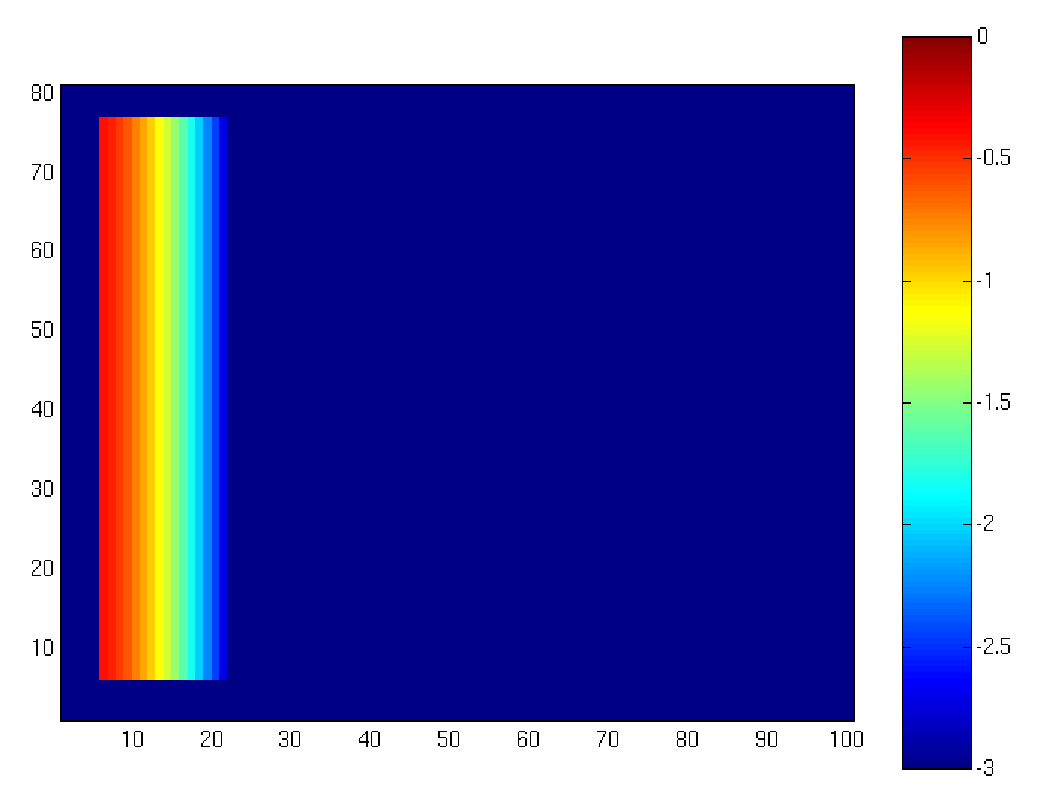
\epsfig{width=3in,file=Code/Fdtd-multidimensional/tfsf-sim3.eps}
  \\
  (a)
  \\
  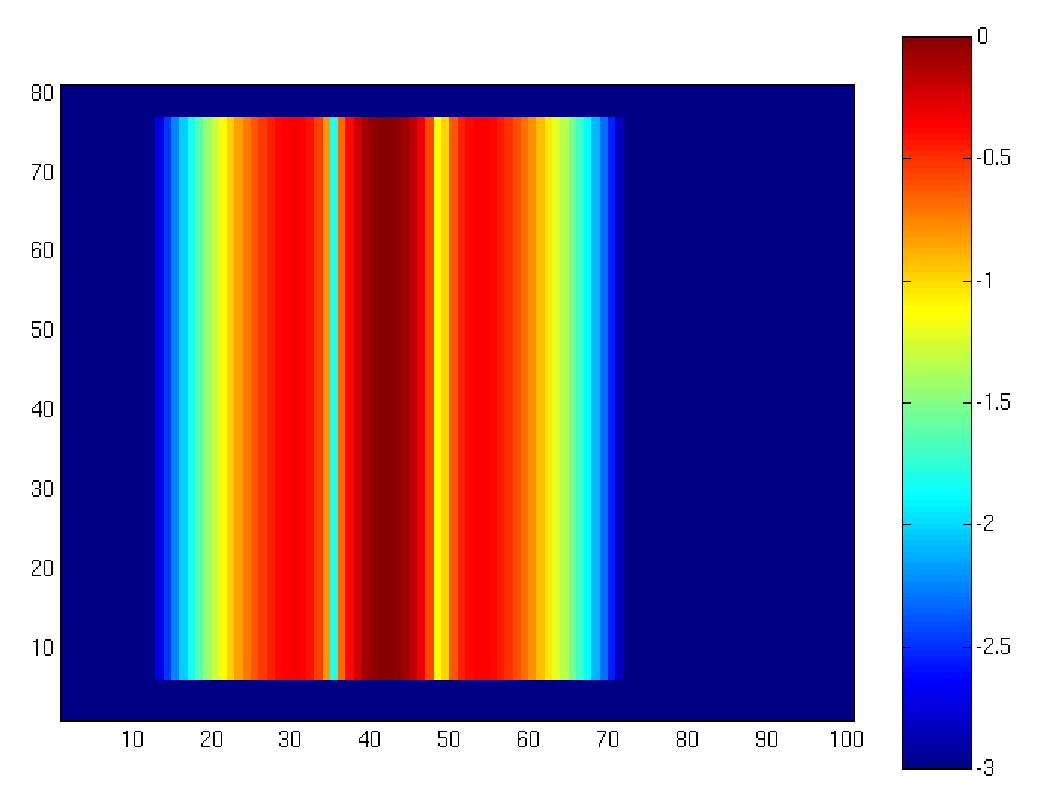
\epsfig{width=3in,file=Code/Fdtd-multidimensional/tfsf-sim10.eps}
  \\
  (b)
  \\
  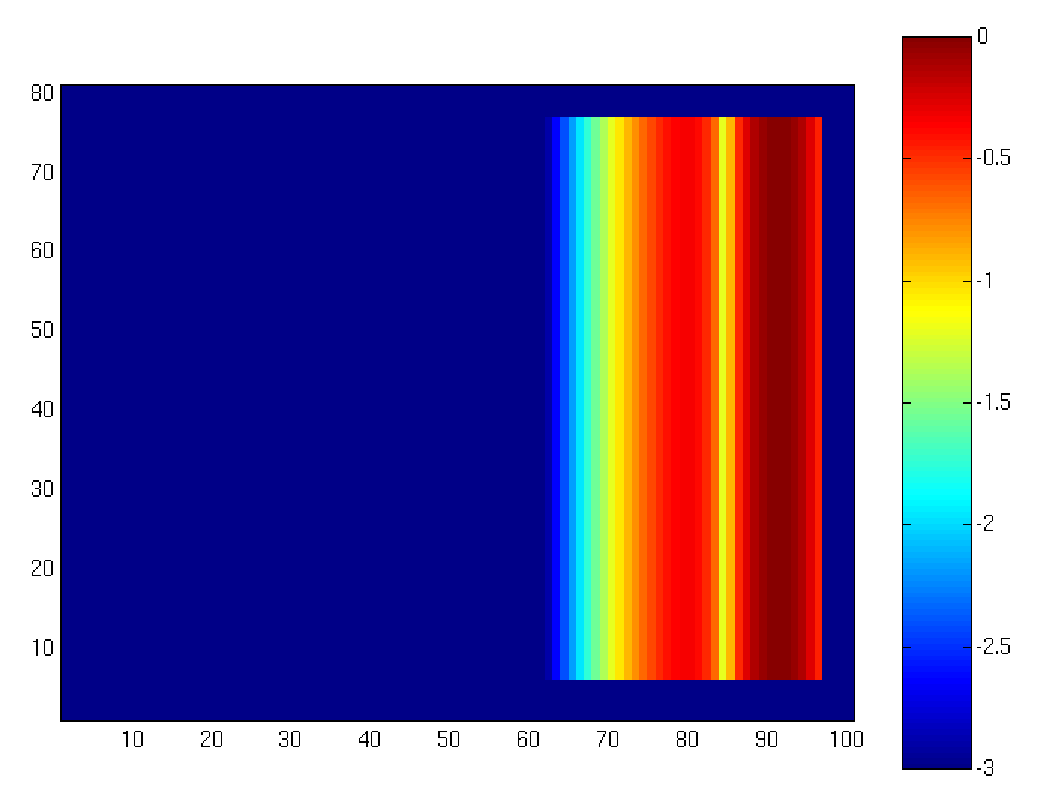
\epsfig{width=3in,file=Code/Fdtd-multidimensional/tfsf-sim17.eps}
  \\
  (c)
  \end{center} \caption{Display of $E_z$ field in a computational
  domain employing a TFSF boundary.  Snapshots are taken at time-steps
  (a) $30$, (b) $100$, and (c) $170$.  The pulsed, plane-wave source
  corresponds to a Ricker wavelet with $30$ points per wavelength at
  its most energetic frequency.}
  \label{fig:tfsfDemo}
\end{figure}

In Fig.\ \ref{fig:tfsfDemo}(a) the incident field is seen to have
entered the left side of the TF region.  There is an abrupt
discontinuity in the field as one cross the TFSF boundary.  This
discontinuity is visible to the left of the TF region as well as along
a portion of the top and bottom of the region.  In Fig.\
\ref{fig:tfsfDemo}(b) the pulse is nearly completely within the TF
region.  In Fig.\ \ref{fig:tfsfDemo}(c) the incident pulse has
encountered the right side of the TF region.  At this point the
incident field seemingly disappears!  The corrections to the fields at
the right side of the boundary are such that the incident field does
not escape the TF region.

Figure \ref{fig:tfsfPecDemo} shows three snapshots of a computational
domain that is similar to the one shown in Fig.\ \ref{fig:tfsfDemo}.
The only difference is that a PEC plate has been put into the grid.
The plate is realized by setting to zero the $E_z$ nodes along a
vertical line.  This line of nodes is offset $20$ cells from the left
side of the computational domain and runs vertically from $20$ cells
from the bottom of the domain to $20$ cells from the top.  (The way in
which one models a PEC in 2D grids will be discussed further in Sec.\
\ref{sec:tmzTezPec}.)

Second-order ABC's are used to terminate the grid.  (In Fig.\
\ref{fig:tfsfDemo} the fields were normalized to $1.0$.  In 
Fig.\ \ref{fig:tfsfPecDemo} they have been normalized to $2.0$.)
\begin{figure}
  \begin{center}
  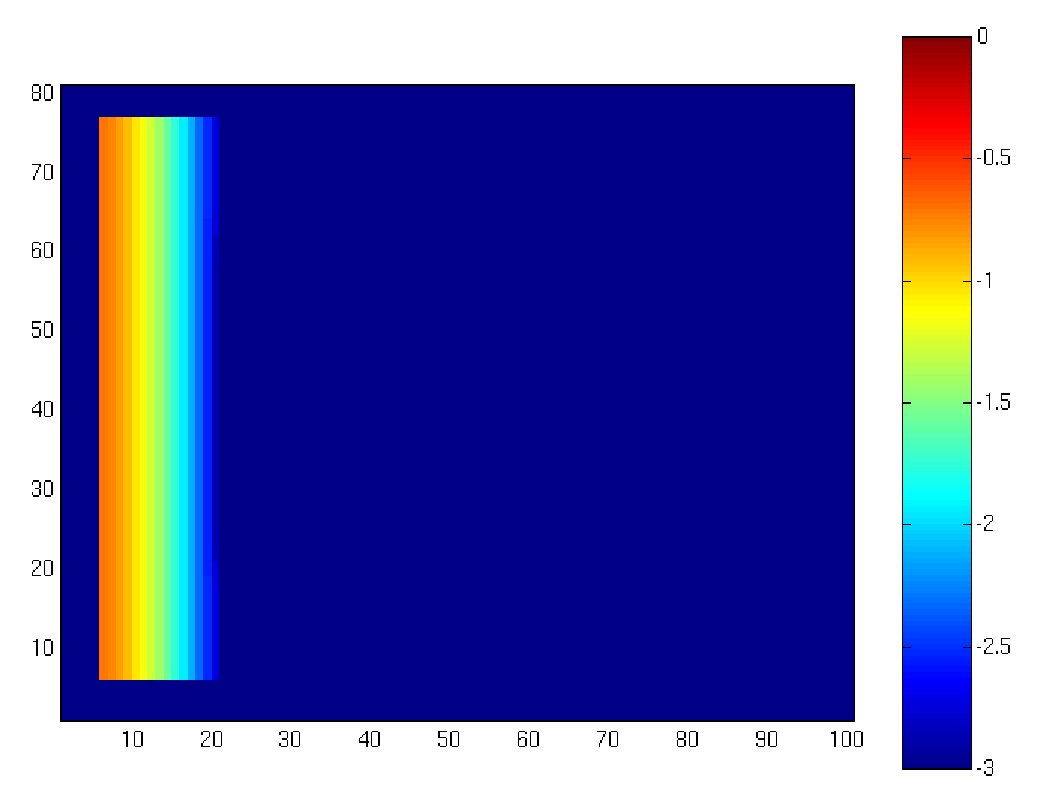
\epsfig{width=3in,file=Code/Fdtd-multidimensional/pec-sim3.eps} \\
  (a) \\
  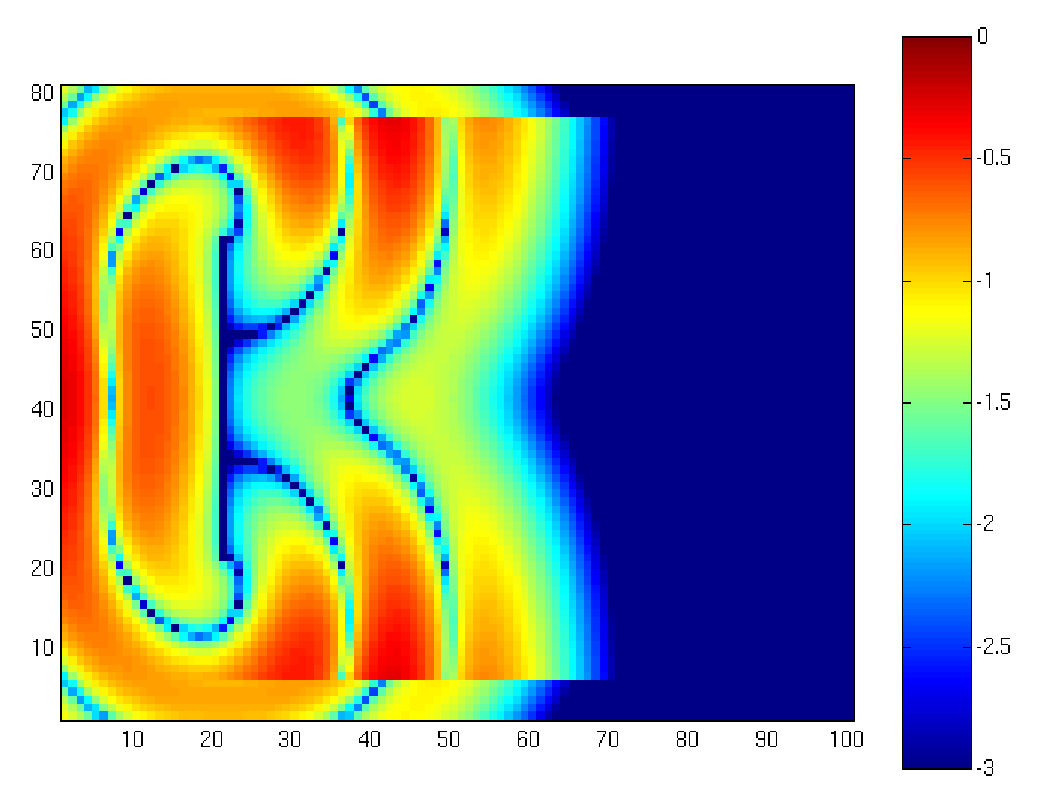
\epsfig{width=3in,file=Code/Fdtd-multidimensional/pec-sim10.eps} \\
  (b) \\
  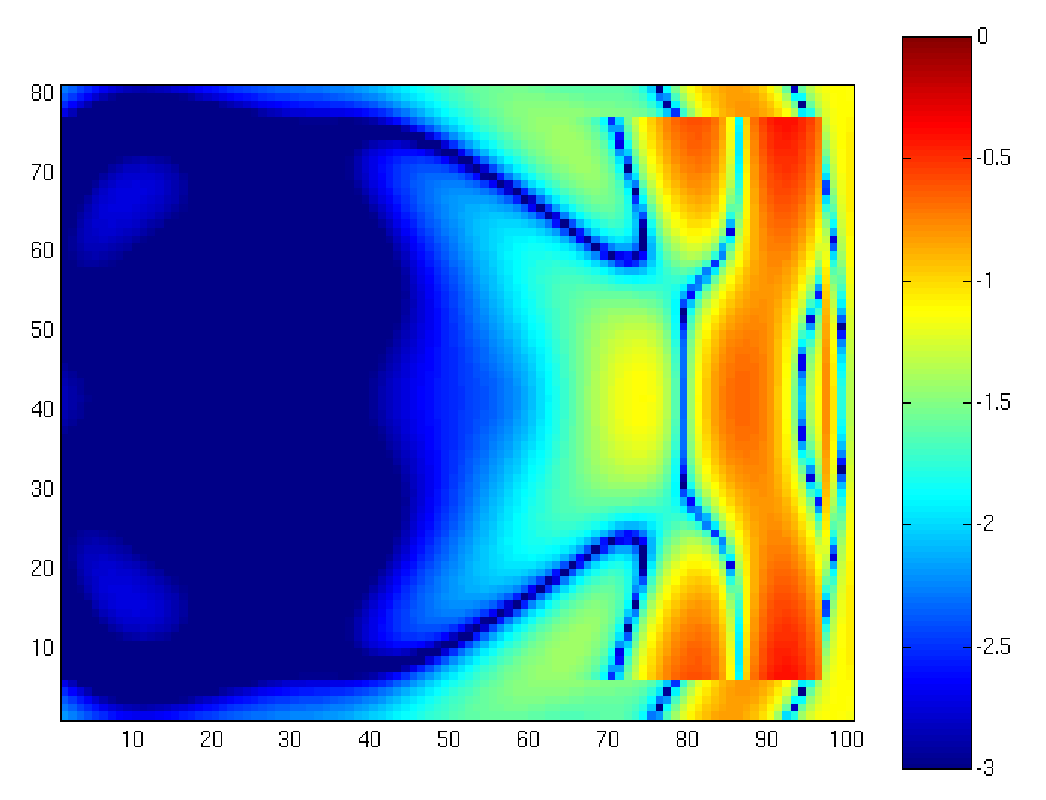
\epsfig{width=3in,file=Code/Fdtd-multidimensional/pec-sim17.eps} \\
  (c) \end{center} \caption{Display of $E_z$ field in a computational
  domain employing a TFSF boundary.  There is a PEC vertical plate
  which is realized by setting to zero the $E_z$ field over a lines
  that is $41$ cells high and $20$ cells from the left edge of the
  computational domain.  Snapshots are taken at time steps (a) $30$,
  (b) $100$, and (c) $170$.  A second-order ABC is used to terminate
  the grid.}  \label{fig:tfsfPecDemo}
\end{figure}

In Fig.\ \ref{fig:tfsfPecDemo}(a) the incident field has just barely
reached the plate.  There is no scattering evident yet and
hence no scattered fields are visible in the SF region.  In Fig.\
\ref{fig:tfsfPecDemo}(b) the interaction of the field with the plate
is obvious.  One can see how the fields have diffracted around the
edges of the plate.  As can be seen, the field scattered from the
plate has had time to propagate into the SF region.  Figure
\ref{fig:tfsfPecDemo}(c) also shows the non-zero field in the SF
region (together with the total field throughout the TF region).  The
ABC's must absorb the scattered field, but they do not have to contend
with the incident field since, as shown in Fig.\
\ref{fig:tfsfDemo}, the incident field never escapes the TF region
(but, of course, the scattered field at any point along the edge of
the computational domain could be as large or larger than the incident
field---it depends on how the scatterer scatters the field).

The organization of code used to generate the results shown in Fig.\
\ref{fig:tfsfPecDemo} is depicted in Fig.\ \ref{fig:tmzdemo2}.  The
header files are not shown.  The contents of the files {\tt
updatetmz.c}, {\tt ricker.c}, and {\tt snapshot2d.c} are unchanged
from the previous section (refer to Programs \ref{pro:updatetmz},
\ref{pro:ricker}, and \ref{pro:snap2d}, respectively).  The file {\tt
gridtmz.c} has changed only slightly from the code shown in Program
\ref{pro:gridtmz} in that a line of electric-field update coefficients
are now set to zero corresponding to the location of the PEC.  Since
this change is so minor, this file is not presented here.  The header
files {\tt fdtd-alloc1.h}, {\tt fdtd-grid1.h} and {\tt
fdtd-macro-tmz.h} are also unchanged from the previous section (refer
to Programs \ref{pro:fdtdalloc1h}, \ref{pro:fdtdgrid1h}, and
\ref{pro:fdtdmacrotmzh}).

\begin{figure}
  \begin{center}
  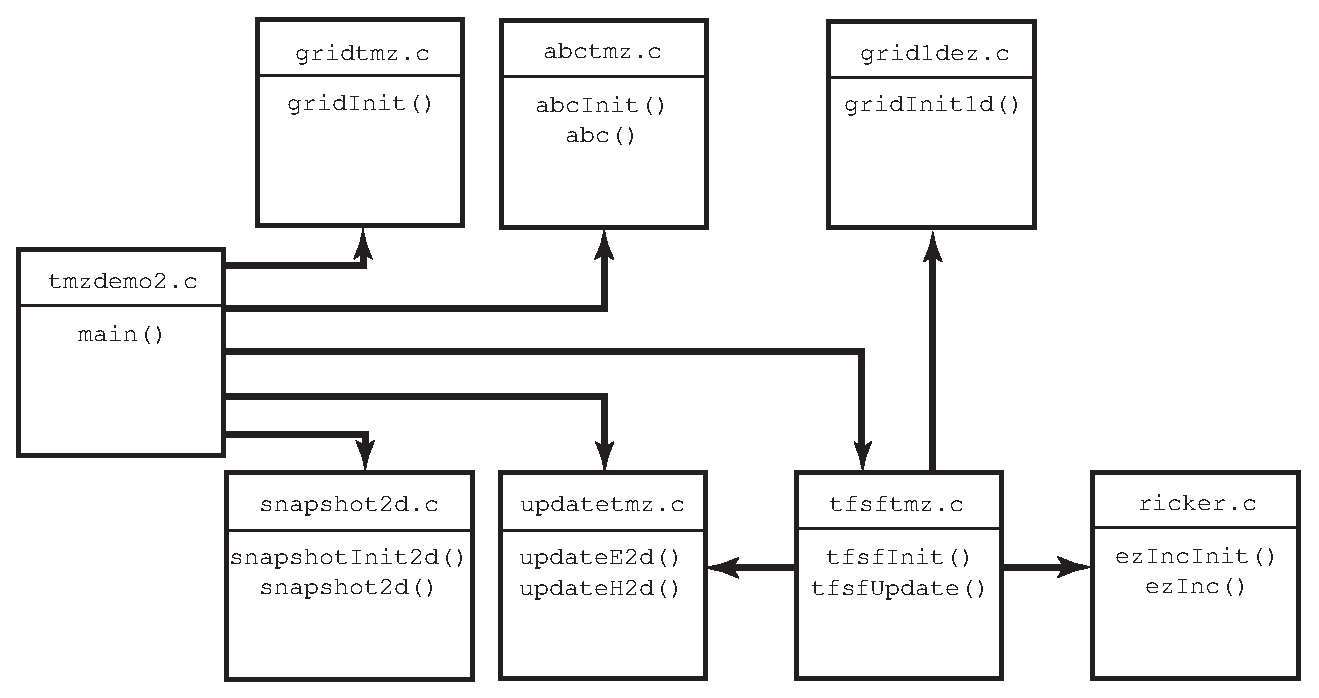
\epsfig{width=5in,file=Figures/Fdtd-multidimensional/tmzdemo2-files.eps}
  \end{center} \caption{Organization of files associated with a TM$^z$
  simulation that employs a TFSF boundary and a second-order ABC.  The header files are
  not shown.}  \label{fig:tmzdemo2}
\end{figure}

The contents of {\tt tmzdemo2.c} are shown in Program
\ref{pro:tmzdemo2}.  This program differs from Program
\ref{pro:tmzdemo1} only in the call to the TFSF and ABC functions.
Also, a different prototype header file is included.  These difference
are shown in bold.

\begin{program}
{\tt tmzdemo2.c} 
Program to perform a TM$^z$ simulation where the field is introduced
via a TFSF boundary and the grid is terminated with a second-order
ABC.  The differences between this code and Program \ref{pro:tmzdemo1}
are shown in bold.
\label{pro:tmzdemo2}
\codemiddle
\begin{lstlisting}
/* TMz simulation with a TFSF boundary and a second-order ABC. */

#include "fdtd-alloc1.h"
#include "fdtd-macro-tmz.h" 
/*b*/#include "fdtd-proto2.h" /*n*/

int main()
{
  Grid *g;

  ALLOC_1D(g, 1, Grid); // allocate memory for grid /*@ \label{tmzdemo2A} @*/
  gridInit(g);          // initialize 2D grid

  abcInit(g);           // initialize ABC
  tfsfInit(g);          // initialize TFSF boundary
  snapshotInit2d(g);    // initialize snapshots

  /* do time stepping */
  for (Time = 0; Time < MaxTime; Time++) { /*@ \label{tmzdemo2C} @*/
    updateH2d(g);       // update magnetic fields 
/*b*/    tfsfUpdate(g);      // apply TFSF boundary    /*n*/
    updateE2d(g);       // update electric fields 
/*b*/    abc(g);             // apply ABC              /*n*/
    snapshot2d(g);      // take a snapshot (if appropriate)
  } // end of time-stepping

  return 0;
}
\end{lstlisting}
\end{program}

After initialization of the 2D grid in line \ref{tmzdemo2A}, the ABC,
TFSF, and snapshot functions are initialized.  Time-stepping begins in
line \ref{tmzdemo2C}.  Within the time-stepping loop, first the
magnetic fields are updated.  As already mentioned, the function {\tt
updateH2d()} is unchanged from before.  We merely pass to it the the
{\tt Grid} pointer {\tt g}.  Next, the function {\tt tfsfUpdate()} is
used to update the fields adjacent to the TFSF boundary.  This
function takes (the 2D {\tt Grid} pointer) {\tt g} as an argument.  As we will
see, the TFSF function also keeps track of an auxiliary 1D that is
completely hidden from {\tt main()}.  The electric fields are then
updated, the ABC is applied, and a snapshot is generated (if the
time-step is appropriate).

The header file {\tt fdtd-proto2.h} is shown in Program
\ref{pro:fdtdproto2}.  The only substantial changes from Program
\ref{pro:fdtdproto1} are the addition of the prototypes for the TFSF,
ABC functions, and a function used to initialize the 1D grid.

\begin{program}
{\tt fdtd-proto2.h} Header file that now includes the prototypes for
the TFSF and ABC functions.  The differences between this file and
\ref{pro:fdtdproto1} are shown in bold.
\label{pro:fdtdproto2}
\codemiddle
\begin{lstlisting}
/*b*/#ifndef _FDTD_PROTO2_H
#define _FDTD_PROTO2_H /*n*/

#include "fdtd-grid1.h"

/* Function prototypes */
/*b*/void abcInit(Grid *g);
void abc(Grid *g);

void gridInit1d(Grid *g); /*n*/
void gridInit(Grid *g);

void snapshotInit2d(Grid *g);
void snapshot2d(Grid *g);

/*b*/void tfsfInit(Grid *g);
void tfsfUpdate(Grid *g); /*n*/

void updateE2d(Grid *g);
void updateH2d(Grid *g);

#endif
\end{lstlisting}
\end{program}

The code to implement the TFSF boundary is shown in Program\
\ref{pro:tfsftmz}.  There are five global variables in this program.
The four declared on lines \ref{tfsftmzA} and \ref{tfsftmzB} give the
indices of the first and last points in the TF region.  The global
variable {\tt g1}, declared on line \ref{tfsftmzC}, is a {\tt Grid}
pointer that will be used for the auxiliary 1D grid.

The function {\tt tfsfInit()} starts by allocating space for {\tt g1}.
Once that space has been allocated we could set the Courant number,
the maximum number of time steps, and the size of the grid.  However,
it is important that these values match, at least in some ways, the
value of the 2D grid that has already been declared.  Thus, in line
\ref{tfsftmzD}, the contents of the 2D grid structure are copy to the
1D grid structure.  To accomplish this copying the C function {\tt
memcpy()} is used.  This function takes three arguments: the
destination memory address, the source memory address, and the amount
of memory to be copied.  After this copying has been completed, there
are some things about the {\tt g1} which are incorrect.  For example,
its {\tt type} corresponds to a 2D TM$^z$ grid.  Also, the pointers
for its arrays are the same as those for the 2D grid.  We do not want
the 1D grid writing to the same arrays as the 2D grid!  Therefore
these values within the {\tt Grid} pointer {\tt g1} need to be fix and
this is accomplished with the grid-initialization function {\tt
gridInit1D()} called in \ref{tfsftmzE}.  We will consider the details
of that function soon.  Just prior to returning, {\tt tfsfInit()}
initializes the source function by calling {\tt ezIncInit()}.

As we saw in the {\tt main()} function in Program \ref{pro:tmzdemo2},
{\tt tfsfUpdate()} is called once per time-step, after the magnetic
fields have been updated and before the electric field is updated.
Note that the fields throughout the grid are not consistent until
after the electric field has been updated in the 2D grid (i.e., after
step three in the algorithm described on page
\pageref{page:tfsfUpdateAlgorithm}).  This is because just prior to
calling {\tt tfsfUpdate()} the magnetic fields have not been corrected
to account for the TFSF boundary.  Just after {\tt tfsfUpdate()} has
returned the electric field has been corrected in anticipation of the
next update.

\begin{program}
{\tt tfsftmz.c}
Source code to implement a TFSF boundary for a TM$^z$ grid.  The
incident field is assumed to propagate along the $x$ direction and is
calculated using an auxiliary 1D simulation.
\label{pro:tfsftmz}
\codemiddle
\begin{lstlisting}
#include <string.h>  // for memcpy
#include "fdtd-macro-tmz.h"
#include "fdtd-proto2.h"
#include "fdtd-alloc1.h"
#include "ezinc.h"

static int firstX = 0, firstY, // indices for first point in TF region /*@\label{tfsftmzA}@*/
           lastX, lastY;       // indices for last point in TF region  /*@\label{tfsftmzB}@*/

static Grid *g1;  // 1D auxilliary grid  /*@\label{tfsftmzC}@*/

void tfsfInit(Grid *g) {

  ALLOC_1D(g1, 1, Grid);       // allocate memory for 1D Grid
  memcpy(g1, g, sizeof(Grid)); // copy information from 2D array /*@\label{tfsftmzD}@*/
  gridInit1d(g1);              // initialize 1d grid/*@\label{tfsftmzE}@*/

  printf("Grid is %d by %d cell.\n", SizeX, SizeY);
  printf("Enter indices for first point in TF region: ");
  scanf(" %d %d", &firstX, &firstY);
  printf("Enter indices for last point in TF region: ");
  scanf(" %d %d", &lastX, &lastY);

  ezIncInit(g); // initialize source function

  return;
}

void tfsfUpdate(Grid *g) {
  int mm, nn;

  // check if tfsfInit() has been called
  if (firstX <= 0) {
    fprintf(stderr,
      "tfsfUpdate: tfsfInit must be called before tfsfUpdate.\n"
      "            Boundary location must be set to positive value.\n");
    exit(-1);
  }

  // correct Hy along left edge
  mm = firstX - 1;
  for (nn = firstY; nn <= lastY; nn++)
    Hy(mm, nn) -= Chye(mm, nn) * Ez1G(g1, mm + 1);
  
  // correct Hy along right edge
  mm = lastX;
  for (nn = firstY; nn <= lastY; nn++)
    Hy(mm, nn) += Chye(mm, nn) * Ez1G(g1, mm);

  // correct Hx along the bottom
  nn = firstY - 1;
  for (mm = firstX; mm <= lastX; mm++)
    Hx(mm, nn) += Chxe(mm, nn) * Ez1G(g1, mm);

  // correct Hx along the top
  nn = lastY;
  for (mm = firstX; mm <= lastX; mm++)
    Hx(mm, nn) -= Chxe(mm, nn) * Ez1G(g1, mm);

  updateH2d(g1);    // update 1D magnetic field  /*@\label{tfsftmzF}@*/
  updateE2d(g1);    // update 1D electric field
  Ez1G(g1, 0) = ezInc(TimeG(g1), 0.0); // set source node
  TimeG(g1)++;      // increment time in 1D grid

  /* correct Ez adjacent to TFSF boundary */
  // correct Ez field along left edge
  mm = firstX;  /*@ \label{tfsftmzG} @*/
  for (nn = firstY; nn <= lastY; nn++)
    Ez(mm, nn) -= Cezh(mm, nn) * Hy1G(g1, mm - 1);
  
  // correct Ez field along right edge
  mm = lastX;
  for (nn = firstY; nn <= lastY; nn++)
    Ez(mm, nn) += Cezh(mm, nn) * Hy1G(g1, mm);
  
  // no need to correct Ez along top and bottom since
  // incident Hx is zero

  return;
}
\end{lstlisting}
\end{program}

The function {\tt tfsfUpdate()}, which is called once per time-step,
starts by ensuring that the initialization function has been called.
It then corrects $H_y$ along the left and right edges and $H_x$ along
the top and bottom edges.  Then, in line \ref{tfsftmzF}, the magnetic
field in the 1D grid is updated, then the 1D electric field.  Then the
source is realized by hard-wiring the first electric-field node in the
1D grid to the source function (in this case a Ricker wavelet).  This
is followed by incrementing the time-step in the 1D grid.  Now that
the 1D grid has been updated, starting in line \ref{tfsftmzG}, the
electric fields adjacent to the TFSF boundary are corrected.
Throughout {\tt tfsfUpdate()} any macro that pertains to {\tt g1} must
explicitly specify the {\tt Grid} as an argument.

The function used to initialize the 1D grid is shown in Program
\ref{pro:grid1dez}.  After inclusion of the appropriate header files, 
{\tt NLOSS} is defined to be $20$.  The 1D grid is terminated with a
lossy layer rather than an ABC\@.  {\tt NLOSS} represents the number of
nodes in this lossy region.

\begin{program}
{\tt grid1dez.c}
Initialization function for the 1D auxilliary grid used by the TFSF
function to calculate the incident field.
\label{pro:grid1dez}
\codemiddle
\begin{lstlisting}
#include <math.h>
#include "fdtd-macro-tmz.h"
#include "fdtd-alloc1.h"

#define NLOSS     20   // number of lossy cells at end of 1D grid
#define MAX_LOSS  0.35 // maximum loss factor in lossy layer /*@\label{grid1dezX}@*/

void gridInit1d(Grid *g) {
  double imp0 = 377.0, depthInLayer, lossFactor;
  int mm;

  SizeX += NLOSS;    // size of domain /*@\label{grid1dezA}@*/
  Type = oneDGrid;   // set grid type  /*@\label{grid1dezB}@*/

  ALLOC_1D(g->hy,   SizeX - 1, double);    /*@\label{grid1dezC}@*/
  ALLOC_1D(g->chyh, SizeX - 1, double);
  ALLOC_1D(g->chye, SizeX - 1, double);
  ALLOC_1D(g->ez,   SizeX, double);
  ALLOC_1D(g->ceze, SizeX, double);
  ALLOC_1D(g->cezh, SizeX, double);    /*@\label{grid1dezD}@*/
  
  /* set the electric- and magnetic-field update coefficients */
  for (mm = 0; mm < SizeX - 1; mm++) {    /*@\label{grid1dezE}@*/
    if (mm < SizeX - 1 - NLOSS) {
      Ceze1(mm) = 1.0;
      Cezh1(mm) = Cdtds * imp0;
      Chyh1(mm) = 1.0;
      Chye1(mm) = Cdtds / imp0;
    } else {
      depthInLayer = mm - (SizeX - 1 - NLOSS) + 0.5;
      lossFactor = MAX_LOSS * pow(depthInLayer / NLOSS, 2);
      Ceze1(mm) = (1.0 - lossFactor) / (1.0 + lossFactor);
      Cezh1(mm) = Cdtds * imp0 / (1.0 + lossFactor);
      depthInLayer += 0.5;
      lossFactor = MAX_LOSS * pow(depthInLayer / NLOSS, 2);
      Chyh1(mm) = (1.0 - lossFactor) / (1.0 + lossFactor);
      Chye1(mm) = Cdtds / imp0 / (1.0 + lossFactor);
    }
  }

  return;
}
\end{lstlisting}
\end{program}

Recall that in {\tt tfsfInit()} the values from the 2D grid were
copied to the 1D grid (ref.\ line \ref{tfsftmzD} of Program
\ref{pro:tfsftmz}).  Thus at the start of this function the value of
{\tt SizeX} is set to that of the 2D grid.  (The value of {\tt SizeY}
is also set to that of the 2D grid, but this value is ignored in the
context of a 1D grid.)  In line \ref{grid1dezA} the size is increased by
the number of nodes in the lossy layer.  This is the final size of the
1D grid: $20$ cells greater than the $x$ dimension of the 2D grid.

The grid type is specified as being a {\tt oneDGrid} in line
\ref{grid1dezB}.  (There is no need to set the Courant number since that
was copied from the 2D grid.)  This is followed by memory allocation
for the various arrays in lines \ref{grid1dezC} to \ref{grid1dezD}.

The update-equation coefficients are set by the for-loop that begins
on line \ref{grid1dezE}.  (The final electric-field node does not have
its coefficient set as it will not be updated.)  The region of the 1D
grid corresponding to the width of the 2D grid is set to free space.
Recalling the discussion of Sec.\ \ref{sec:loss}, the remainder of the
grid is set to a lossy layer where the electric and magnetic loss are
matched so that the characteristic impedance remains that of free
space.  However, unlike in Sec.\ \ref{sec:loss}, here the amount of
loss is small at the start of the layer and grows towards the end of
the grid: The loss increases quadratically as one approaches the end
of the grid.  The maximum ``loss factor'' (which corresponds to
$\sigma\Delt/2\epsilon$ in the electric-field update equations or
$\sigma_m\Delt/2\mu$ in the magnetic-field update equations) is set by
the {\tt \#define} statement on line \ref{grid1dezX} to $0.35$.  By
gradually ramping up the loss, the reflections associated with having
an abrupt change in material constants can be greatly reduced.
Further note that although the loss factor associated with the
electric and magnetic fields are matches, because the electric and
magnetic fields are spatially offset, the loss factor that pertains at
electric and magnetic field nodes differ even when they have the same
spatial index.  The loss factor is based on the variable {\tt
  depthInLayer} which represents how deep a particular node is within
the lossy layer.  The greater the depth, the greater the loss.

Finally, the file {\tt abctmz.c} is shown in Program \ref{pro:abctmz}.
There are four arrays used to store the old values of field needed by
the ABC---one array for each side of the grid.  For each node along
the edge of the grid, six values must be stored.  Thus the arrays that
store values along the left and right sides have a total of $6 \times$
{\tt SizeY} elements while the arrays that store values along the top
and bottom have $6 \times$ {\tt SizeX} elements.  Starting on line
\ref{abctmzA} four macros are defined that simplify accessing the
elements of these arrays.  The macros take three arguments.  One
arguments specifies displacement along the edge of the grid.  Another
specifies the displacement into the interior.  The third argument
specifies the number of steps back in time.

\begin{program}
{\tt abctmz.c}  Function to apply a second-order ABC to a TM$^z$ grid.
\label{pro:abctmz}
\codemiddle
\begin{lstlisting}
/* Second-order ABC for TMz grid. */
#include <math.h>
#include "fdtd-alloc1.h"
#include "fdtd-macro-tmz.h"

/* Define macros for arrays that store the previous values of the
 * fields.  For each one of these arrays the three arguments are as
 * follows:
 *
 *   first argument:  spatial displacement from the boundary
 *   second argument: displacement back in time
 *   third argument:  distance from either the bottom (if EzLeft or
 *                    EzRight) or left (if EzTop or EzBottom) side
 *                    of grid
 *                    
 */
#define EzLeft(M, Q, N)   ezLeft[(N) * 6 + (Q) * 3 + (M)] /*@\label{abctmzA}@*/
#define EzRight(M, Q, N) ezRight[(N) * 6 + (Q) * 3 + (M)]
#define EzTop(N, Q, M)       ezTop[(M) * 6 + (Q) * 3 + (N)]
#define EzBottom(N, Q, M) ezBottom[(M) * 6 + (Q) * 3 + (N)]

static int initDone = 0;
static double coef0, coef1, coef2;
static double *ezLeft, *ezRight, *ezTop, *ezBottom;

void abcInit(Grid *g) {   /*@\label{abctmzB}@*/
  double temp1, temp2;
  
  initDone = 1;

  /* allocate memory for ABC arrays */
  ALLOC_1D(ezLeft, SizeY * 6, double);
  ALLOC_1D(ezRight, SizeY * 6, double);
  ALLOC_1D(ezTop, SizeX * 6, double);
  ALLOC_1D(ezBottom, SizeX * 6, double);

  /* calculate ABC coefficients */
  temp1 = sqrt(Cezh(0, 0) * Chye(0, 0)); /*@\label{abctmzC}@*/
  temp2 = 1.0 / temp1 + 2.0 + temp1;
  coef0 = -(1.0 / temp1 - 2.0 + temp1) / temp2;
  coef1 = -2.0 * (temp1 - 1.0 / temp1) / temp2;
  coef2 = 4.0 * (temp1 + 1.0 / temp1) / temp2;

  return;
} 

void abc(Grid *g) /*@\label{abctmzD}@*/
{
  int mm, nn;

  /* ABC at left side of grid */
  for (nn = 0; nn < SizeY; nn++) {
    Ez(0, nn) = coef0 * (Ez(2, nn) + EzLeft(0, 1, nn))
     + coef1 * (EzLeft(0, 0, nn) + EzLeft(2, 0, nn)
                - Ez(1, nn) - EzLeft(1, 1, nn))
     + coef2 * EzLeft(1, 0, nn) - EzLeft(2, 1, nn);

    /* memorize old fields */ 
    for (mm = 0; mm < 3; mm++) {
      EzLeft(mm, 1, nn) = EzLeft(mm, 0, nn);
      EzLeft(mm, 0, nn) = Ez(mm, nn);
    }
  }
  
  /* ABC at right side of grid */
  for (nn = 0; nn < SizeY; nn++) {
    Ez(SizeX - 1, nn) = coef0 * (Ez(SizeX - 3, nn) + EzRight(0, 1, nn))
     + coef1 * (EzRight(0, 0, nn) + EzRight(2, 0, nn)
                - Ez(SizeX - 2, nn) - EzRight(1, 1, nn))
     + coef2 * EzRight(1, 0, nn) - EzRight(2, 1, nn);
  
    /* memorize old fields */
    for (mm = 0; mm < 3; mm++) {
      EzRight(mm, 1, nn) = EzRight(mm, 0, nn);
      EzRight(mm, 0, nn) = Ez(SizeX - 1 - mm, nn);
    }
  }

  /* ABC at bottom of grid */
  for (mm = 0; mm < SizeX; mm++) {
    Ez(mm, 0) = coef0 * (Ez(mm, 2) + EzBottom(0, 1, mm))
     + coef1 * (EzBottom(0, 0, mm) + EzBottom(2, 0, mm)
                - Ez(mm, 1) - EzBottom(1, 1, mm))
     + coef2 * EzBottom(1, 0, mm) - EzBottom(2, 1, mm);

    /* memorize old fields */ 
    for (nn = 0; nn < 3; nn++) {
      EzBottom(nn, 1, mm) = EzBottom(nn, 0, mm);
      EzBottom(nn, 0, mm) = Ez(mm, nn);
    }
  }
  
  /* ABC at top of grid */
  for (mm = 0; mm < SizeX; mm++) {
    Ez(mm, SizeY - 1) = coef0 * (Ez(mm, SizeY - 3) + EzTop(0, 1, mm))
     + coef1 * (EzTop(0, 0, mm) + EzTop(2, 0, mm)
                - Ez(mm, SizeY - 2) - EzTop(1, 1, mm))
     + coef2 * EzTop(1, 0, mm) - EzTop(2, 1, mm);
  
    /* memorize old fields */
    for (nn = 0; nn < 3; nn++) {
      EzTop(nn, 1, mm) = EzTop(nn, 0, mm);
      EzTop(nn, 0, mm) = Ez(mm, SizeY - 1 - nn);
    }
  }

  return;
}
\end{lstlisting}
\end{program}

The initialization function starting on line \ref{abctmzB} allocates
space for the arrays and calculates the coefficients used by the ABC.
It is assumed the grid is uniform along the edge and the coefficients
are calculated based on the parameters that pertain at the first node
in the grid (as indicated by the statements starting on line \ref{abctmzC}).

The {\tt abc()} function, which starts on line \ref{abctmzD} and is
called once per time step, systematically applies the ABC to each node
along the edge of the grid.  After the ABC is applied to an edge, the
``old'' stored values are updated.


%%%%%%%%%%%%%%%%%%%%%%%%%%%%%%%%%%%%%%%%%%%%%%%%%%%%%%%%%%%%%%%%%%%%%%%%%%%
\section{TE$^z$ Polarization}

In TE$^z$ polarization the non-zero fields are $E_x$, $E_y$, and
$H_z$, i.e., the electric field is transverse to the $z$ direction.
The fields may vary in the $x$ and $y$ directions but are invariant in
$z$.  These fields, and the corresponding governing equations, are
completely decoupled from those of TM$^z$ polarization.  The governing
equations are
\begin{eqnarray}
  \sigma E_x + \epsilon\frac{\partial E_x}{\partial t} &=&
    \frac{\partial H_z}{\partial y},  \label{eq:TEzX}
  \\
  \sigma E_y + \epsilon\frac{\partial E_y}{\partial t} &=&
    -\frac{\partial H_z}{\partial x}, \label{eq:TEzY}
  \\
  -\sigma_m H_z - \mu\frac{\partial H_z}{\partial t} &=&
     \frac{\partial E_y}{\partial x}
    -\frac{\partial E_x}{\partial y}. \label{eq:TEzZ}
\end{eqnarray}

As usual, space-time is discretized so that
\refeq{eq:TEzX}--\refeq{eq:TEzZ} can be expressed in
terms of finite-differences.  From these difference equations the
future fields can be expressed in terms of past fields.  The following
notation will be used:
\begin{eqnarray}
  E_x(x,y,t) \!&=&\! E_x(m\Delx, n\Dely, q\Delt) =
          \fdtd{E_x}{m,n}{q},  \\
  E_y(x,y,t) \!&=&\! E_y(m\Delx, n\Dely, q\Delt) =
          \fdtd{E_y}{m,n}{q}  \\
  H_z(x,y,t) \!&=&\! H_z(m\Delx, n\Dely, q\Delt) = \fdtd{H_z}{m,n}{q}.
\end{eqnarray}
As before the indices $m$, $n$, and $q$ specify the step in the $x$,
$y$, and $t$ ``directions.''

A suitable arrangement of nodes is shown in Fig.\ \ref{fig:tezGrid}.
The triangularly shaped dashed lines in the lower left of the grid
enclose nodes which would have the same indices in a computer
program.

\begin{figure}
  \begin{center}
  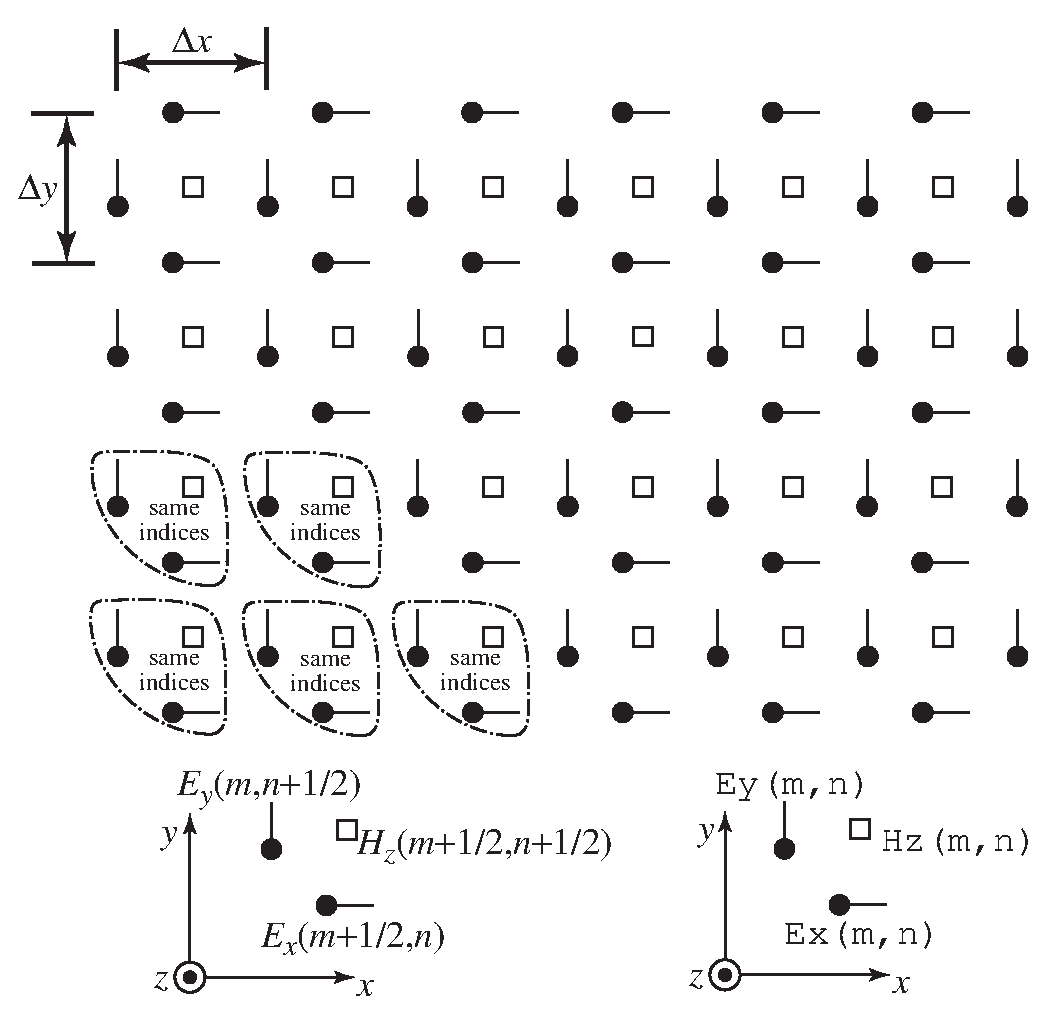
\epsfig{width=5in,file=Figures/Fdtd-multidimensional/te-fdtd-grid.eps}
  \end{center} \caption{Spatial arrangement of electric- and
  magnetic-field nodes for TE$^z$ polarization.  The magnetic-field
  nodes are shown as squares and the electric-field nodes are circles
  with a line that indicates the orientation of the field component.
  The somewhat triangularly shaped dashed lines indicate groupings of
  nodes which have the same array indices. This grouping is repeated
  throughout the grid.  However, at the top of the grid the ``group''
  only contains an $E_x$ node and on the right side of the grid the
  group only contains an $E_y$ node.  The diagram at the bottom left
  of the figure indicates nodes with their offsets given explicitly in
  the spatial arguments whereas the diagram at the bottom right
  indicates how the same nodes would be specified in a computer
  program where the offsets are understood implicitly.}
  \label{fig:tezGrid}
\end{figure}

Note that the grid is terminated such that there are tangential
electric field nodes adjacent to the boundary.  (When it comes to the
application of ABC's, these are the nodes to which the ABC would be
applied.)  When we say a TE$^z$ grid has dimensions $M\times N$, the
arrays are dimensioned as follows: $E_x$ is $(M-1)\times N$, $E_y$ is
$M\times (N-1)$, and $H_z$ is $(M-1)\times (N-1)$.  Therefore,
although the grid is described as $M\times N$, no array actually has
these dimensions!  Each magnetic-field node has four adjacent
electric-field nodes that ``swirl'' about it.  One can think of these
four nodes as defining a square with the magnetic field at the center
of the square (if the grid is not uniform, the square becomes a
rectangle).  An $M\times N$ grid would consist of $(M-1)\times (N-1)$
complete squares.

The way in which the TE$^z$ arrays are dimensioned may seem odd but it
is done with an eye toward having a consistent grid in three
dimensions.  As an indication of where we will ultimately end up, we
can overlay a TM$^z$ and TE$^z$ grid as shown in Fig.\
\ref{fig:teTmOverlay}.  As will be shown in the discussion of 3D
grids, a 3D grid is essentially layers of TM$^z$ and TE$^z$ grids
which are offset from each other in the $z$ direction.  The update
equations of these offset grids will have to be modified to account
for variations in the $z$ directions.  This modification will provide
the coupling between the TM$^z$ and TE$^z$ grids which is lacking in
2D.

\begin{figure}
  \begin{center}
  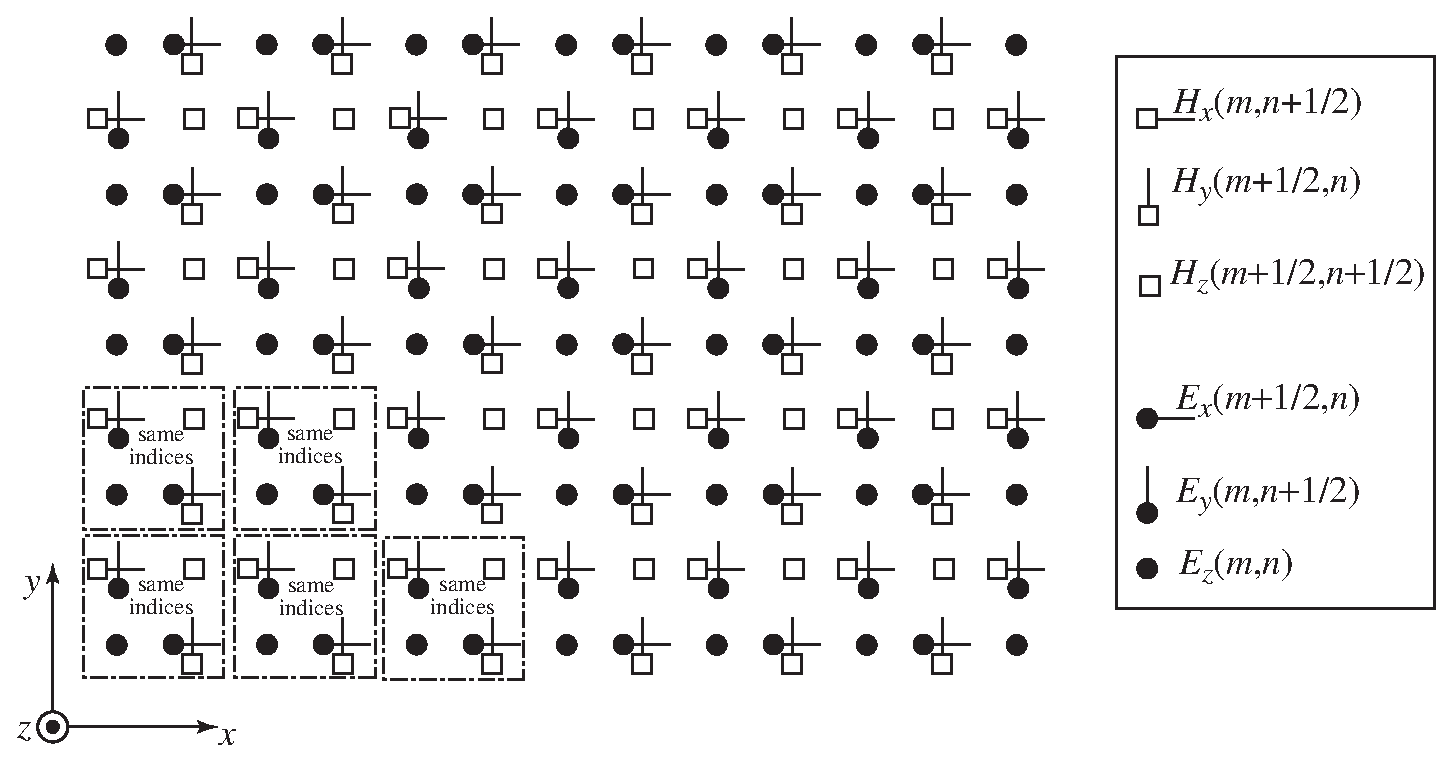
\epsfig{width=6.25in,file=Figures/Fdtd-multidimensional/te-tm-overlay.eps}
  \end{center} 
  \caption{Superposition of a TM$^z$ and TE$^z$ grid.  The symbols
  used for the nodes is as before.  The dashed boxes enclose nodes
  which have the same indices.  Although this is nominally identified
  as an $M\times N$ grid, only the $E_z$ array has $M\times N$ nodes.}
  \label{fig:teTmOverlay}
\end{figure}

Given the governing equations \refeq{eq:TEzX}--\refeq{eq:TEzZ} and the
arrangement of nodes shown in Fig.\ \ref{fig:tezGrid}, the $H_z$ update
equation is
\begin{eqnarray}
  \fdtdh{H_z}{m+\half,n+\half}{q+\half} &=&
  \frac{1-\frac{\sigma_m\Delt}{2\mu}}{1+\frac{\sigma_m\Delt}{2\mu}}
  \fdtdh{H_z}{m+\half,n+\half}{q-\half}
 \nonumber\\
  && \hspace{-.35in}\mbox{} -
  \frac{1}{1+\frac{\sigma_m\Delt}{2\epsilon}}
  \left(
    \frac{\Delt}{\epsilon\Delx}
    \left\{
      \fdtdh{E_y}{m+1,n+\half}{q} - \fdtdh{E_y}{m,n+\half}{q}
    \right\} \right.\nonumber\\
  && \hspace{.366in}\left.\mbox{}-
    \frac{\Delt}{\mu\Dely}
    \left\{
      \fdtdh{E_x}{m+\half,n+1}{q} - \fdtdh{E_x}{m+\half,n}{q}
    \right\}
  \right).
\end{eqnarray}
The electric-field update equations are
\begin{eqnarray}
  \fdtdh{E_x}{m+\half,n}{q+1} &=&
   \frac{1-\frac{\sigma\Delt}{2\epsilon}}{1+\frac{\sigma\Delt}{2\epsilon}}
   \fdtd{E_x}{m+\half,n}{q} \nonumber\\
   && \hspace{-.75in}\mbox{} +
   \frac{1}{1+\frac{\sigma\Delt}{2\epsilon}}
    \frac{\Delt}{\epsilon\Dely}
    \left(\fdtdh{H_z}{m+\half,n+\half}{q+\half}-
          \fdtdh{H_z}{m+\half,n-\half}{q+\half}\right),\\
  \fdtdh{E_y}{m,n+\half}{q+1} &=&
   \frac{1-\frac{\sigma\Delt}{2\epsilon}}{1+\frac{\sigma\Delt}{2\epsilon}}
   \fdtd{E_y}{m,n+\half}{q}\nonumber\\
   && \hspace{-.75in}\mbox{} -
   \frac{1}{1+\frac{\sigma\Delt}{2\epsilon}}
   \frac{\Delt}{\epsilon\Delx}
    \left(\fdtd{H_z}{m+\half,n+\half}{q+\half}-
          \fdtd{H_z}{m-\half,n+\half}{q+\half}\right).
\end{eqnarray}

Similar to the TM$^z$ case, we assume a uniform grid and define the
following quantities
\begin{eqnarray}
\chzh(m+1/2,n+1/2) &=&
  \left.
    \frac{1-\frac{\sigma_m\Delt}{2\mu}}{1+\frac{\sigma_m\Delt}{2\mu}}
  \right|_{(m+1/2)\Delx,(n+1/2)\Dely}, \\
\chze(m+1/2,n+1/2) &=&
  \left.
    \frac{1}{1+\frac{\sigma_m\Delt}{2\mu}}\frac{\Delt}{\mu\delta}
  \right|_{(m+1/2)\Delx,(n+1/2)\Dely}, \\
\cexe(m+1/2,n) &=&
  \left.
    \frac{1-\frac{\sigma\Delt}{2\epsilon}}{1+\frac{\sigma\Delt}{2\epsilon}}
  \right|_{(m+1/2)\Delx,n\Dely}, \\
\cexh(m+1/2,n) &=&
  \left.
    \frac{1}{1+\frac{\sigma_m\Delt}{2\epsilon}}\frac{\Delt}{\epsilon\delta}
  \right|_{(m+1/2)\Delx,n\Dely}, \\
\ceye(m,n+1/2) &=& 
  \left.
  \frac{1-\frac{\sigma\Delt}{2\epsilon}}{1+\frac{\sigma\Delt}{2\epsilon}}
  \right|_{m\Delx,(n+1/2)\Dely}, \\
\ceyh(m,n+1/2) &=& 
  \left.
  \frac{1}{1+\frac{\sigma\Delt}{2\epsilon}}
    \frac{\Delt}{\epsilon\delta}
  \right|_{m\Delx,(n+1/2)\Dely}.
\end{eqnarray}
By discarding the explicit offsets of one-half (but leaving them as
implicitly understood) the update equations can be written in a form
suitable for implementation in a computer.  Because of the arrangement
of the nodes, this ``discarding'' implies that sometimes the one-half
truly is discarded and sometimes it should be replaced with unity.
The distinction is whether or not the one-half indicates the nodes on
the right side of the update equation are within the same grouping of
cells as the node on the left side of the equation.  If they are, the
one-half is truly discarded.  If they are not, the node on the right
side of the update equation must have its index reflect which group of
cells it is within relative to the node on the left side of the
equation.  The resulting equations are
\begin{code}
  Hz(m, n) = Chzh(m, n) * Hz(m, n) +
     Chze(m, n) * ((Ex(m, n + 1) - Ex(m, n)) -
                   (Ey(m + 1, n) - Ey(m, n)));
  Ex(m, n) = Cexe(m, n) * Ex(m, n) +
     Cexh(m, n) * (Hz(m, n) - Hz(m, n - 1));
  Ey(m, n) = Ceye(m, n) * Ey(m, n) -
     Ceyh(m, n) * (Hz(m, n) - Hz(m - 1, n));
\end{code}

A TFSF boundary can be incorporated in a TE$^z$ grid.  Conceptually
the implementation is the same as has been shown in 1D and in the
TM$^z$ grid.  Nodes that are tangential to the boundary will have a
neighboring node on the other side of the boundary.  The incident
field will have to be either added to or subtracted from that
neighboring node to obtain consistent equations.  A portion of a
TE$^z$ grid showing the TFSF boundary is shown in Fig.\
\ref{fig:teTfsf}.  We will specify the size of the TF region as
indicated in the figure.  Indices that specify the start of the TF
region correspond to the first $E_x$ and $E_y$ nodes which are in the
TF region.  Referring to Figs.\ \ref{fig:tmzTfsf} and
\ref{fig:teTmOverlay}, these indices would also correspond to the
first $E_z$ node in the TF region.  The indices which specify the end
of the TF region correspond to $E_x$ and $E_y$ nodes which are
actually in the SF region.  These two nodes, as shown in Fig.\
\ref{fig:teTmOverlay}, are not tangential to the TFSF boundary and
hence do to have to be corrected.  However, note that the $E_z$ node
in the overlain grid that has these indices does lie in the TF region
(and does, when dealing with a 3D or TM$^z$ grid, have to be corrected
to account for the presence of the boundary).

\begin{figure}
  \begin{center}
  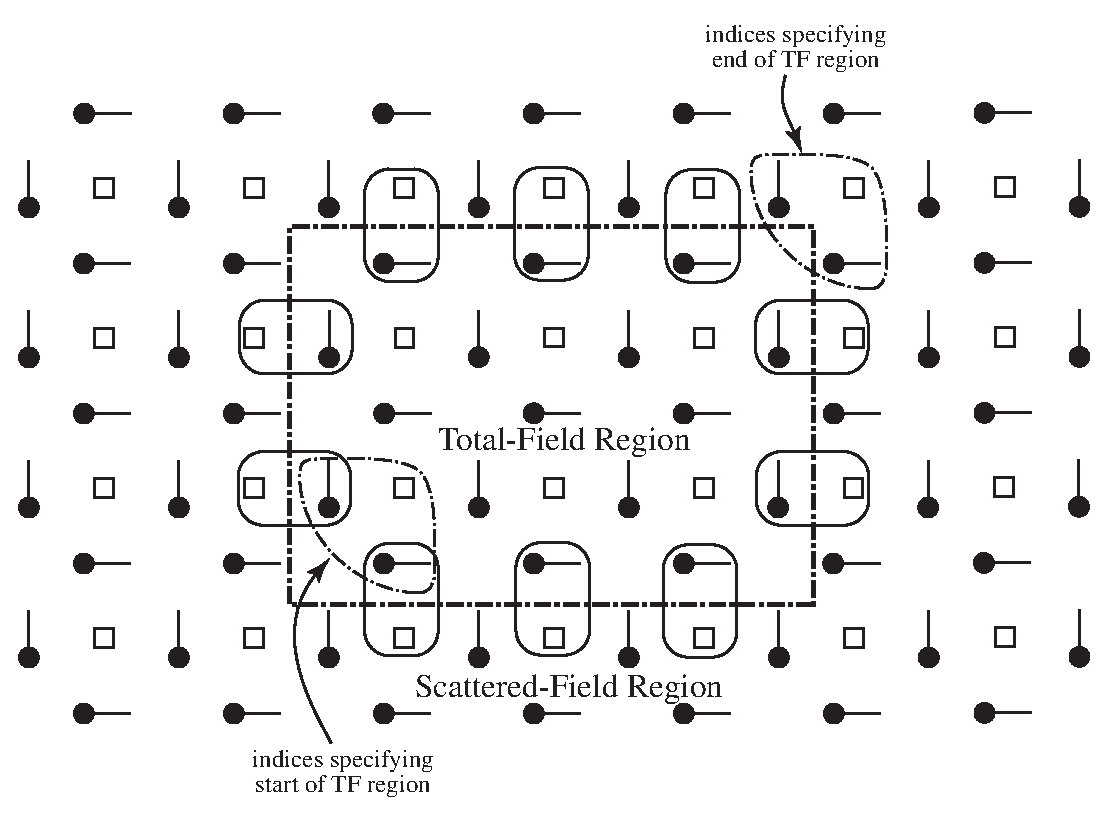
\epsfig{width=5in,file=Figures/Fdtd-multidimensional/te-fdtd-tfsf.eps}
  \end{center} 
  \caption{TFSF boundary in a TE$^z$ grid.  The rounded boxes indicate
  the nodes that have a neighboring node on the other side of the
  boundary and hence have to have their update equations corrected.}
  \label{fig:teTfsf}
\end{figure}

\section{PEC's in TE$^z$ and TM$^z$ Simulations \label{sec:tmzTezPec}}

When modeling a PEC in a TM$^z$ grid, if an $E_z$ node falls within
the PEC, it is set to zero.  Figure \ref{fig:tmPec} shows a portion of
a TM$^z$ grid that depicts how $E_z$ would set to zero.  The curved
boundary is the surface of the PEC and it is assumed that the PEC
extends down and to the right of this boundary.  The $E_z$ nodes which
would be set to zero are indicated with gray boxes.  Although the goal
is to model a continuously varying boundary, the discrete nature of
the FDTD grid gives rise to a ``staircased'' approximation of the
surface.

When we say a node is ``set to zero'' this could mean various things.
For example, it may mean that the field is initially zero and then
never updated.  It could mean that it is updated, but the update
coefficients are set to zero.  Or, it could even mean that the field
is updated with non-zero coefficients, but then additional code is
used to set the field to zero each time-step.  The means by which a
field is set to zero is not particularly important to us right now.

\begin{figure}
  \begin{center}
  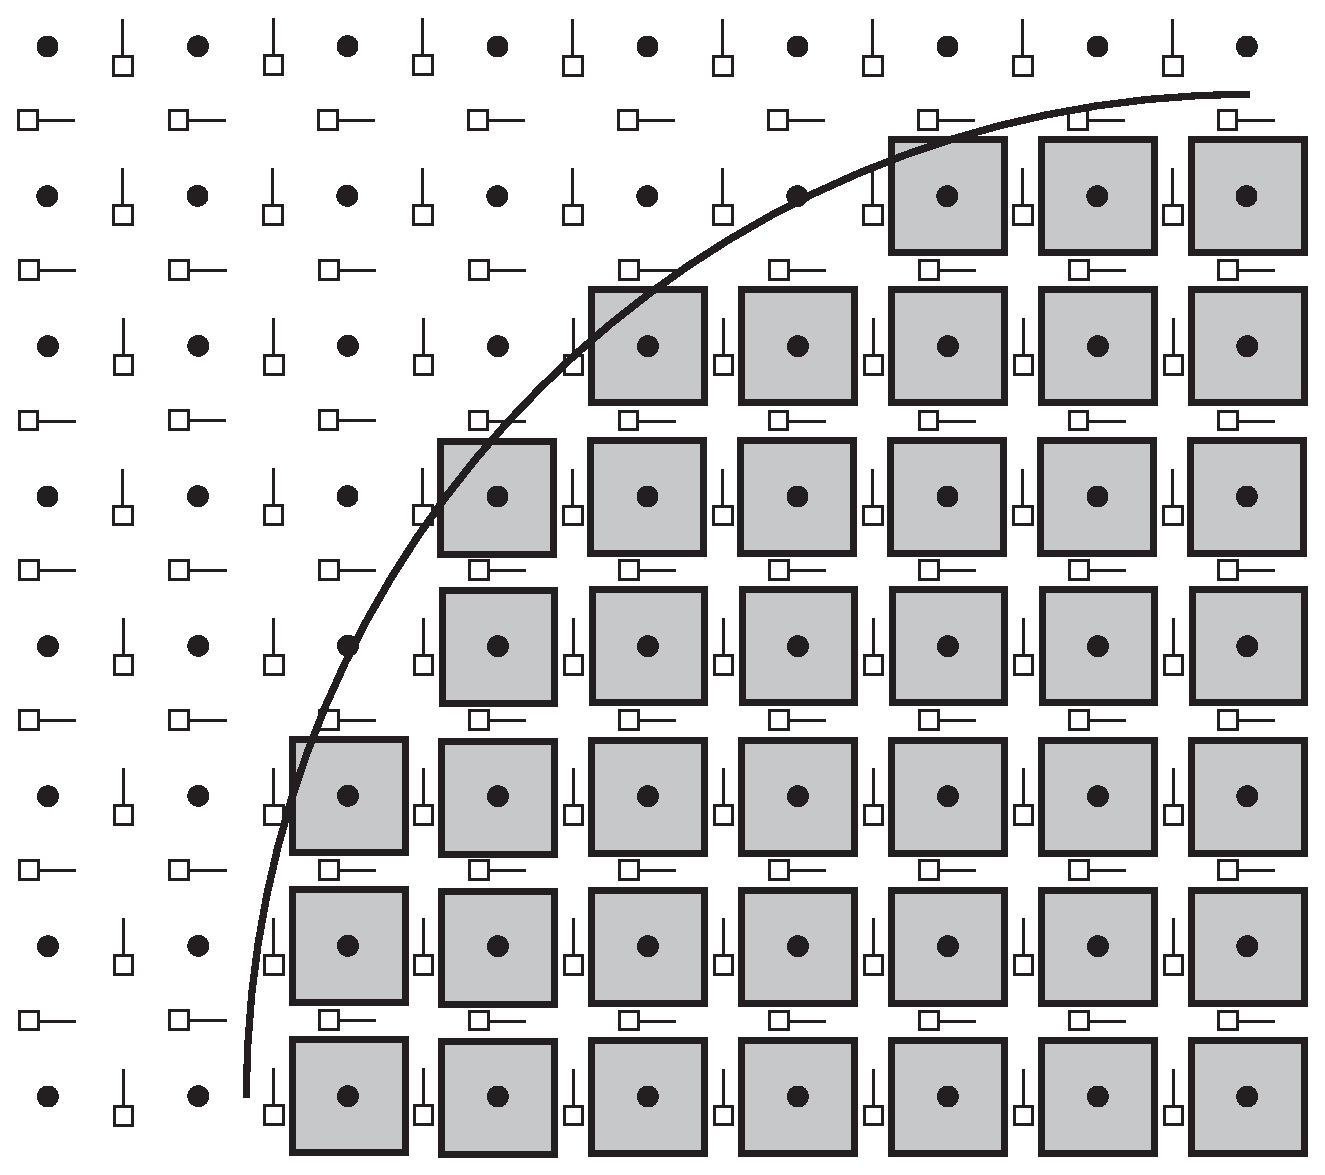
\epsfig{width=5in,file=Figures/Fdtd-multidimensional/tm-pec.eps}
  \end{center} 
  \caption{TM$^z$ grid with a PEC object.  The PEC is assumed to exist
  below and to the right of the curved boundary.  The PEC is realized
  by setting to zero the $E_z$ nodes that fall within the PEC.  The
  nodes that would be set to zero are surrounded by gray boxes.}
  \label{fig:tmPec}
\end{figure}

A thin PEC plate can be modeled in a TM$^z$ grid by setting to zero
nodes along a vertical or horizontal line.  If the physical plate
being modeled is not aligned with the grid, one would have to zero
nodes in a manner that approximates the true slope of the plate.
Again, this would yield a staircased approximate to the true surface.
(One may have to be careful to ensure that there are no ``gaps'' in
the model of a thin PEC that is not aligned with the grid.  Fields
should only be able to get from one side of the PEC to the other by
propagating around the ends of the PEC.)

In a TE$^z$ grid, the realization of a PEC is slightly more
complicated.  For a PEC object which has a specified cross section,
one should not merely set to zero the electric-field nodes that fall
within the boundary of the PEC (as was done in the TM$^z$ case).
Instead, one should consider the PEC as consisting of a collection of
patches of metal.  If an $H_z$ node falls within the PEC, then four
surrounding electric-field nodes should be set to zero.  Thus, if an
$H_z$ node is in the PEC we fill the square surrounding that node with
PEC and this causes the four surrounding electric field nodes to be
zero.  The TE$^z$ representation of a PEC object is depicted in Fig.\
\ref{fig:tePec}.  The object is the same as shown in Fig.\
\ref{fig:tmPec}.  In both figures the curved boundary is a portion of
a circle that is center on what would correspond to the location of an
$E_z$ node (regardless of whether or not an $E_z$ node is actually
present).  The nodes that are set to zero are enclosed in gray
rectangles.

\begin{figure}
  \begin{center}
  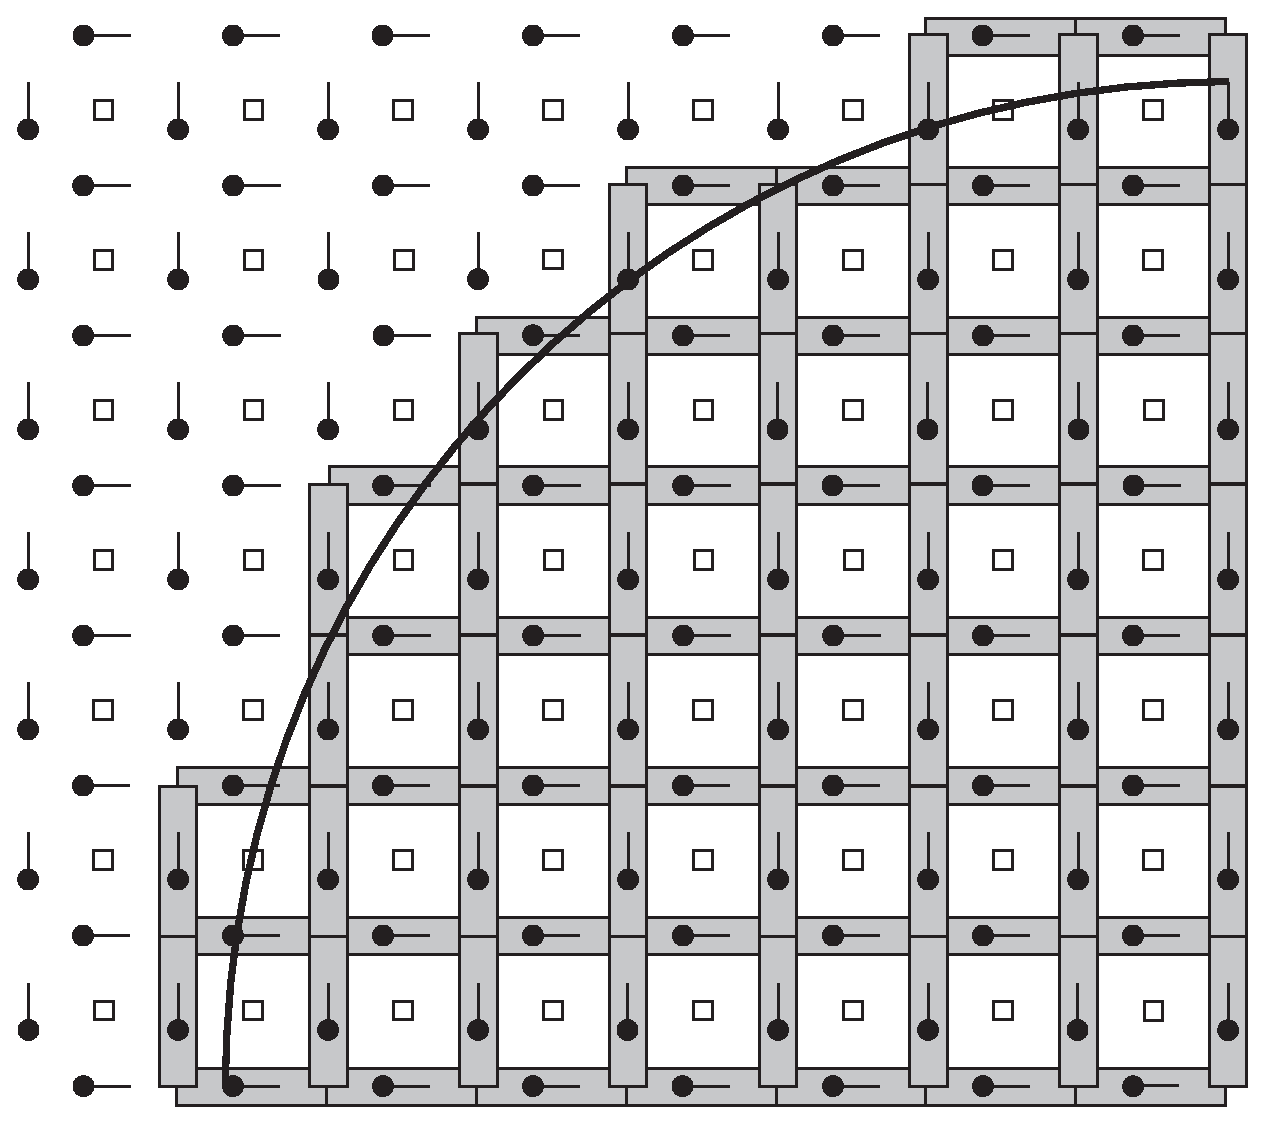
\epsfig{width=5in,file=Figures/Fdtd-multidimensional/te-pec.eps}
  \end{center} \caption{TE$^z$ grid with a PEC object.  The PEC is
  assumed to exist below and to the right of the curved boundary.  The
  PEC is realized be setting to zero any electric field which has a
  neighboring $H_z$ node within the PEC.  The nodes that would be set
  to zero are surrounded by gray rectangles.}  \label{fig:tePec}
\end{figure}

A horizontal PEC plate would be implemented by zeroing a horizontal
line of $E_x$ nodes while a vertical plate would be realized by
zeroing a vertical line of $E_y$ nodes.  A tilted plate would be
realized as a combination of zeroed $E_x$ and $E_y$ nodes.

For both TE$^z$ and TM$^z$ grids, all the magnetic fields are updated
in the usual way.  Magnetic fields are oblivious to the presence of
PEC's.

\section{TE$^z$ Example}

In this section we present the computer code to model a circular PEC
scatterer in a TE$^z$ grid.  The scatterer is illuminated by a pulsed
plane wave that is introduced via a TFSF boundary.  We will use a grid
that is nominally $92$ by $82$ (keeping in mind that for TE$^z$
polarization none of the field arrays will actually have these
dimensions).  The code is organized in essentially the same way as was
the TM$^z$ code presented in Sec.\ \ref{sec:tmzTfsf}.

The PEC scatterer is assumed to have a radius of $12$ cells and be
centered on an $H_z$ node.  The indices of the center are $(45,40)$.
The PEC is realized by checking if an $H_z$ node is within the circle
(specifically, if the distance from the center to the node is less
than the radius).  As we will see, if an $H_z$ is within the circle,
the four surrounding electric-field nodes are set to zero by setting
the corresponding update coefficients to zero.

Program \ref{pro:tezdemo} contains the {\tt main()} function.  Other
than the difference of one header file, this program is identical to
the TM$^z$ code presented in Program \ref{pro:tmzdemo2}.  However,
despite similar names, the functions that are called
here differ from those used by Program \ref{pro:tmzdemo2}---different
files are linked together for the different simulations.

\begin{program}
{\tt tezdemo.c} The {\tt main()} function for a simulation involving a
TE$^z$ grid.
\label{pro:tezdemo}
\codemiddle
\begin{lstlisting}
/* TEz simulation with a TFSF boundary and a second-order ABC. */

#include "fdtd-alloc1.h"
#include "fdtd-macro-tez.h" 
#include "fdtd-proto2.h"

int main()
{
  Grid *g;

  ALLOC_1D(g, 1, Grid); // allocate memory for grid
  gridInit(g);        // initialize 2D grid

  abcInit(g);         // initialize ABC
  tfsfInit(g);        // initialize TFSF boundary
  snapshotInit2d(g);  // initialize snapshots

  /* do time stepping */
  for (Time = 0; Time < MaxTime; Time++) {
    updateH2d(g);     // update magnetic fields 
    tfsfUpdate(g);    // apply TFSF boundary
    updateE2d(g);     // update electric fields 
    abc(g);           // apply ABC
    snapshot2d(g);    // take a snapshot (if appropriate)
  } // end of time-stepping

  return 0;
}
\end{lstlisting}
\end{program}

The code to construct the TE$^z$ grid is shown in Program
\ref{pro:gridtezpec}, i.e., the code to set the elements of the {\tt
Grid} pointer {\tt g}.  The simulation is run at the Courant limit of
$1/\sqrt{2}$ as shown in line \ref{gridtezpecA}.  Between lines
\ref{gridtezpecB} and \ref{gridtezpecC} the update coefficients for
all the electric field nodes are set to that of free space.  Then,
starting at line \ref{gridtezpecD}, each $H_z$ node is checked to see
if it is within the PEC scatterer.  If it is, the coefficients for the
surrounding nodes are set to zero.  Starting at line \ref{gridtezpecE}
all the magnetic-field coefficients are set to that of free space.
There is no need to change these coefficients to account for the
PEC---the PEC is realized solely by dictating the behavior of the
electric field.

\begin{program}
{\tt gridtezpec.c} Function to initialize a TE$^z$ grid.  A circular
PEC scatterer is present.
\label{pro:gridtezpec}
\codemiddle
\begin{lstlisting}
#include "fdtd-macro-tez.h"
#include "fdtd-alloc1.h"
#include <math.h>

void gridInit(Grid *g) {
  double imp0 = 377.0;
  int mm, nn;

  /* terms for the PEC scatterer */
  double rad, r2, xLocation, yLocation, xCenter, yCenter;

  Type = teZGrid;
  SizeX = 92;      // size of domain
  SizeY = 82;
  MaxTime = 300;   // duration of simulation
  Cdtds = 1.0 / sqrt(2.0); // Courant number /*@ \label{gridtezpecA} @*/

  ALLOC_2D(g->hz,   SizeX - 1, SizeY - 1, double);
  ALLOC_2D(g->chzh, SizeX - 1, SizeY - 1, double);
  ALLOC_2D(g->chze, SizeX - 1, SizeY - 1, double);

  ALLOC_2D(g->ex,   SizeX - 1, SizeY, double);
  ALLOC_2D(g->cexh, SizeX - 1, SizeY, double);
  ALLOC_2D(g->cexe, SizeX - 1, SizeY, double);

  ALLOC_2D(g->ey,   SizeX, SizeY - 1, double);
  ALLOC_2D(g->ceye, SizeX, SizeY - 1, double);
  ALLOC_2D(g->ceyh, SizeX, SizeY - 1, double);
  
  /* set electric-field update coefficients */
  for (mm = 0; mm < SizeX - 1; mm++) /*@ \label{gridtezpecB} @*/
    for (nn = 0; nn < SizeY; nn++) {
      Cexe(mm, nn) = 1.0;
      Cexh(mm, nn) = Cdtds * imp0;
    }

  for (mm = 0; mm < SizeX; mm++)
    for (nn = 0; nn < SizeY - 1; nn++) {
      Ceye(mm, nn) = 1.0;
      Ceyh(mm, nn) = Cdtds * imp0;
    }                          /*@ \label{gridtezpecC} @*/

  /* Set to zero nodes associated with PEC scatterer.
   * Circular scatterer assumed centered on Hz node
   * at (xCenter, yCenter).  If an Hz node is less than
   * the radius away from this node, set to zero the
   * four electric fields that surround that node. 
   */
  rad = 12;  // radius of circle          /*@ \label{gridtezpecD} @*/
  xCenter = SizeX / 2;
  yCenter = SizeY / 2;
  r2 = rad * rad;  // square of radius
  for (mm = 1; mm < SizeX - 1; mm++) {
    xLocation = mm - xCenter;
    for (nn = 1; nn < SizeY - 1; nn++) {
      yLocation = nn - yCenter;
      if (xLocation * xLocation + yLocation * yLocation < r2) {
	Cexe(mm, nn) = 0.0;
	Cexh(mm, nn) = 0.0;
	Cexe(mm, nn + 1) = 0.0;
	Cexh(mm, nn + 1) = 0.0;
	Ceye(mm + 1, nn) = 0.0;
	Ceyh(mm + 1, nn) = 0.0;
	Ceye(mm, nn) = 0.0;
	Ceyh(mm, nn) = 0.0;
      }
    }
  }

  /* set magnetic-field update coefficients */
  for (mm = 0; mm < SizeX - 1; mm++)     /*@ \label{gridtezpecE} @*/
    for (nn = 0; nn < SizeY - 1; nn++) {
      Chzh(mm, nn) = 1.0;
      Chze(mm, nn) = Cdtds / imp0;
    }

  return;
}
\end{lstlisting}
\end{program}

The header file {\tt fdtd-macro-tez.h} that defines the macros used in
the TE$^z$ simulations is shown in Program \ref{pro:fdtdmacrotez}.
The header files that define the function prototypes ({\tt
fdtd-proto2.h}), the allocation macros ({\tt fdtd-alloc1.h}), and the
{\tt Grid} structure ({\tt fdtd-grid1.h}) are unchanged from before
and hence are not repeated here (refer to Programs
\ref{pro:fdtdproto2}, \ref{pro:fdtdalloc1h}, and \ref{pro:fdtdgrid1h},
respectively).

\begin{program}
{\tt fdtd-macro-tez.h} Macros used for TE$^z$ grids.
\label{pro:fdtdmacrotez}
\codemiddle
\begin{lstlisting}
#ifndef _FDTD_MACRO_TEZ_H
#define _FDTD_MACRO_TEZ_H

#include "fdtd-grid1.h"

/* macros that permit the "Grid" to be specified */
/* one-dimensional grid */
#define Hz1G(G, M)     G->hz[M]
#define Chzh1G(G, M)   G->chzh[M]
#define Chze1G(G, M)   G->chze[M]

#define Ey1G(G, M)     G->ey[M]
#define Ceye1G(G, M)   G->ceye[M]
#define Ceyh1G(G, M)   G->ceyh[M]

/* TEz grid */
#define HzG(G, M, N)     G->hz[(M) * (SizeYG(G) - 1) + (N)]
#define ChzhG(G, M, N) G->chzh[(M) * (SizeYG(G) - 1) + (N)]
#define ChzeG(G, M, N) G->chze[(M) * (SizeYG(G) - 1) + (N)]

#define ExG(G, M, N)     G->ex[(M) * SizeYG(G) + (N)]
#define CexeG(G, M, N) G->cexe[(M) * SizeYG(G) + (N)]
#define CexhG(G, M, N) G->cexh[(M) * SizeYG(G) + (N)]

#define EyG(G, M, N)     G->ey[(M) * (SizeYG(G) - 1) + (N)]
#define CeyeG(G, M, N) G->ceye[(M) * (SizeYG(G) - 1) + (N)]
#define CeyhG(G, M, N) G->ceyh[(M) * (SizeYG(G) - 1) + (N)]

#define SizeXG(G)        G->sizeX
#define SizeYG(G)        G->sizeY
#define SizeZG(G)        G->sizeZ
#define TimeG(G)         G->time
#define MaxTimeG(G)      G->maxTime
#define CdtdsG(G)        G->cdtds
#define TypeG(G)         G->type

/* macros that assume the "Grid" is "g" */
/* one-dimensional grid */
#define Hz1(M)      Hz1G(g, M)
#define Chzh1(M)    Chzh1G(g, M)
#define Chze1(M)    Chze1G(g, M)

#define Ey1(M)      Ey1G(g, M)
#define Ceye1(M)    Ceye1G(g, M)
#define Ceyh1(M)    Ceyh1G(g, M)

/* TEz grid */
#define Hz(M, N)   HzG(g, M, N)
#define Chzh(M, N) ChzhG(g, M, N)
#define Chze(M, N) ChzeG(g, M, N) 

#define Ex(M, N)   ExG(g, M, N)
#define Cexh(M, N) CexhG(g, M, N)
#define Cexe(M, N) CexeG(g, M, N)

#define Ey(M, N)   EyG(g, M, N)
#define Ceye(M, N) CeyeG(g, M, N) 
#define Ceyh(M, N) CeyhG(g, M, N) 

#define SizeX        SizeXG(g)
#define SizeY        SizeYG(g)
#define SizeZ        SizeZG(g)
#define Time         TimeG(g)
#define MaxTime      MaxTimeG(g)
#define Cdtds        CdtdsG(g)
#define Type         TypeG(g)

#endif   /* matches #ifndef _FDTD_MACRO_TEZ_H */
\end{lstlisting}
\end{program}

The functions to update the fields are shown in Program
\ref{pro:updatetez}.  These functions can update fields in either one-
or two-dimensional grid.  If the grid type is {\tt oneDGrid}, here it
is assumed the non-zero fields are $E_y$ and $H_z$.  If that is not
the case, it is assume the grid is a TE$^z$ grid with non-zero fields
$E_x$, $E_y$, and $H_z$.  As has been the case in the past the
electric field updates, starting at line \ref{updatetezB}, update all
the nodes except the nodes at the edge of the grid.  However, since
all the magnetic-field nodes have all their neighbors, as shown
starting on line \ref{updatetezA}, all the magnetic-field nodes in the
grid are updated.

\begin{program}
{\tt updatetez.c}: Functions to update fields in a TE$^z$ grid.
\label{pro:updatetez}
\codemiddle
\begin{lstlisting}
#include "fdtd-macro-tez.h"

/* update magnetic field */
void updateH2d(Grid *g) {
  int mm, nn;

  if (Type == oneDGrid) {

    for (mm = 0; mm < SizeX - 1; mm++)
      Hz1(mm) = Chzh1(mm) * Hz1(mm) 
	- Chze1(mm) * (Ey1(mm + 1) - Ey1(mm));

  } else { 

    for (mm = 0; mm < SizeX - 1; mm++)    /*@ \label{updatetezA} @*/
      for (nn = 0; nn < SizeY - 1; nn++)
	Hz(mm, nn) = Chzh(mm, nn) * Hz(mm, nn) +
	  Chze(mm, nn) * ((Ex(mm, nn + 1) - Ex(mm, nn))
			  - (Ey(mm + 1, nn) - Ey(mm, nn)));
  }

  return;
}

/* update electric field */
void updateE2d(Grid *g) {
  int mm, nn;

  if (Type == oneDGrid) {

    for (mm = 1; mm < SizeX - 1; mm++)
      Ey1(mm) = Ceye1(mm) * Ey1(mm) 
	- Ceyh1(mm) * (Hz1(mm) - Hz1(mm - 1));

  } else { 

    for (mm = 0; mm < SizeX - 1; mm++)    /*@ \label{updatetezB} @*/
      for (nn = 1; nn < SizeY - 1; nn++)
	Ex(mm, nn) = Cexe(mm, nn) * Ex(mm, nn) +
	  Cexh(mm, nn) * (Hz(mm, nn) - Hz(mm, nn - 1));

    for (mm = 1; mm < SizeX - 1; mm++)
      for (nn = 0; nn < SizeY - 1; nn++)
	Ey(mm, nn) = Ceye(mm, nn) * Ey(mm, nn) -
	  Ceyh(mm, nn) * (Hz(mm, nn) - Hz(mm - 1, nn));
  }

  return;
}
\end{lstlisting}
\end{program}

The second-order absorbing boundary condition is realized with the
code in the file {\tt abctez.c} which is shown in Program
\ref{pro:abctez}.  Because of the way the grid is constructed, the ABC
is applied to $E_y$ nodes along the left and right side of the
computational domain and to $E_x$ nodes along the top and bottom.

\begin{program}
{\tt abctez.c}: Contents of file that implements the second-order
absorbing boundary condition for the TE$^z$ grid.
\label{pro:abctez}
\codemiddle
\begin{lstlisting}
/* Second-order ABC for TEz grid. */
#include <math.h>
#include "fdtd-alloc1.h"
#include "fdtd-macro-tez.h"

/* Define macros for arrays that store the previous values of the
 * fields.  For each one of these arrays the three arguments are as
 * follows:
 *
 *   first argument:  spatial displacement from the boundary
 *   second argument: displacement back in time
 *   third argument:  distance from either the bottom (if EyLeft or
 *                    EyRight) or left (if ExTop or ExBottom) side
 *                    of grid
 *                    
 */
#define EyLeft(M, Q, N)    eyLeft[(N) * 6 + (Q) * 3 + (M)]
#define EyRight(M, Q, N)  eyRight[(N) * 6 + (Q) * 3 + (M)]
#define ExTop(N, Q, M)       exTop[(M) * 6 + (Q) * 3 + (N)]
#define ExBottom(N, Q, M) exBottom[(M) * 6 + (Q) * 3 + (N)]

static int initDone = 0;
static double coef0, coef1, coef2;
static double *eyLeft, *eyRight, *exTop, *exBottom;

void abcInit(Grid *g) {
  double temp1, temp2;
  
  initDone = 1;

  /* allocate memory for ABC arrays */
  ALLOC_1D(eyLeft, (SizeY - 1) * 6, double);
  ALLOC_1D(eyRight, (SizeY - 1) * 6, double);
  ALLOC_1D(exTop, (SizeX - 1) * 6, double);
  ALLOC_1D(exBottom, (SizeX - 1) * 6, double);

  /* calculate ABC coefficients */
  temp1  = sqrt(Cexh(0, 0) * Chze(0, 0));
  temp2 = 1.0 / temp1 + 2.0 + temp1;
  coef0 = -(1.0 / temp1 - 2.0 + temp1) / temp2;
  coef1 = -2.0 * (temp1 - 1.0 / temp1) / temp2;
  coef2 = 4.0 * (temp1 + 1.0 / temp1) / temp2;

  return;
} 

void abc(Grid *g)
{
  int mm, nn;

  /* ABC at left side of grid */
  for (nn = 0; nn < SizeY - 1; nn++) {
    Ey(0, nn) = coef0 * (Ey(2, nn) + EyLeft(0, 1, nn))
      + coef1 * (EyLeft(0, 0, nn) + EyLeft(2, 0, nn)
		 - Ey(1, nn) - EyLeft(1, 1, nn))
      + coef2 * EyLeft(1, 0, nn) - EyLeft(2, 1, nn);

    /* memorize old fields */ 
    for (mm = 0; mm < 3; mm++) {
      EyLeft(mm, 1, nn) = EyLeft(mm, 0, nn);
      EyLeft(mm, 0, nn) = Ey(mm, nn);
    }
  }
  
  /* ABC at right side of grid */
  for (nn = 0; nn < SizeY - 1; nn++) {
    Ey(SizeX - 1, nn) = coef0 * (Ey(SizeX - 3, nn) + EyRight(0, 1, nn))
      + coef1 * (EyRight(0, 0, nn) + EyRight(2, 0, nn)
		 - Ey(SizeX - 2, nn) - EyRight(1, 1, nn))
      + coef2 * EyRight(1, 0, nn) - EyRight(2, 1, nn);
    
    /* memorize old fields */
    for (mm = 0; mm < 3; mm++) {
      EyRight(mm, 1, nn) = EyRight(mm, 0, nn);
      EyRight(mm, 0, nn) = Ey(SizeX - 1 - mm, nn);
    }
  }

  /* ABC at bottom of grid */
  for (mm = 0; mm < SizeX - 1; mm++) {
    Ex(mm, 0) = coef0 * (Ex(mm, 2) + ExBottom(0, 1, mm))
      + coef1 * (ExBottom(0, 0, mm) + ExBottom(2, 0, mm)
		 - Ex(mm, 1) - ExBottom(1, 1, mm))
      + coef2 * ExBottom(1, 0, mm) - ExBottom(2, 1, mm);
    
    /* memorize old fields */ 
    for (nn = 0; nn < 3; nn++) {
      ExBottom(nn, 1, mm) = ExBottom(nn, 0, mm);
      ExBottom(nn, 0, mm) = Ex(mm, nn);
    }
  }
  
  /* ABC at top of grid */
  for (mm = 0; mm < SizeX - 1; mm++) {
    Ex(mm, SizeY - 1) = coef0 * (Ex(mm, SizeY - 3) + ExTop(0, 1, mm))
      + coef1 * (ExTop(0, 0, mm) + ExTop(2, 0, mm)
		 - Ex(mm, SizeY - 2) - ExTop(1, 1, mm))
      + coef2 * ExTop(1, 0, mm) - ExTop(2, 1, mm);
    
    /* memorize old fields */
    for (nn = 0; nn < 3; nn++) {
      ExTop(nn, 1, mm) = ExTop(nn, 0, mm);
      ExTop(nn, 0, mm) = Ex(mm, SizeY - 1-nn);
    }
  }
  
  return;
}
\end{lstlisting}
\end{program}

The contents of the file {\tt tfsftez.c} are shown in Program
\ref{pro:tfsftez}.  This closely follows the TFSF code that was used
for the TM$^z$ grid.  Again, a 1D auxiliary grid is used to describe
the incident field.  The 1D grid is available via in the {\tt Grid}
pointer {\tt g1} which is only visible to the functions in this file.
Space for the structure is allocated in line \ref{tfsftezA}.  In the
following line the contents of the 2D structure are copied to the 1D
structure.  This is done to set the size of the grid and the Courant
number.  Then, in line \ref{tfsftezB}, the function {\tt gridInit1d()}
is called to complete the initialization of the 1D grid.

The function {\tt tfsfUpdate()}, which starts on line \ref{tfsftezC},
is called once per time-step.  After ensuring that the initialization
function has been called, the magnetic fields adjacent to the TFSF
boundary are corrected.  Following this, as shown starting on line
\ref{tfsftezD}, the magnetic field in the 1D grid is updated, then the
1D electric field is updated, then the source function is applied to
the first node in the 1D grid, and finally the time-step of the 1D
grid is incremented.  Starting on line \ref{tfsftezE}, the electric
fields in the 2D grid adjacent to the TFSF boundary are corrected.

The header file {\tt ezinctez.h} differs from {\tt ezinc.h} used in
the TM$^z$ code only in that it includes {\tt fdtd-macro-tez.h}
instead of {\tt fdtd-macro-tmz.h}.  Hence it is not shown here nor is
the code used to realize the source function which is a Ricker
wavelet (which is also essentially unchanged from before).

\begin{program}
{\tt tfsftez.c}:  Implementation of a TFSF boundary for a TE$^z$
grid.  The incident field propagates in the $x$ direction and an
auxiliary 1D grid is used to compute the incident field.
\label{pro:tfsftez}
\codemiddle
\begin{lstlisting}
/* TFSF implementation for a TEz grid. */

#include <string.h>  // for memcpy
#include "fdtd-macro-tez.h"
#include "fdtd-proto2.h"
#include "fdtd-alloc1.h"
#include "ezinctez.h"    /*@\label{tfsftezF}@*/

static int firstX = 0, firstY, // indices for first point in TF region 
           lastX, lastY;     // indices for last point in TF region

static Grid *g1;  // 1D auxilliary grid

void tfsfInit(Grid *g) {

  ALLOC_1D(g1, 1, Grid);       // allocate memory for 1D Grid /*@\label{tfsftezA}@*/
  memcpy(g1, g, sizeof(Grid)); // copy information from 2D array
  gridInit1d(g1);            // initialize 1d grid /*@\label{tfsftezB}@*/

  printf("Grid is %d by %d cell.\n", SizeX, SizeY);
  printf("Enter indices for first point in TF region: ");
  scanf(" %d %d", &firstX, &firstY);
  printf("Enter indices for last point in TF region: ");
  scanf(" %d %d", &lastX, &lastY);

  ezIncInit(g); // initialize source function

  return;
}

void tfsfUpdate(Grid *g) { /*@\label{tfsftezC}@*/
  int mm, nn;

  // check if tfsfInit() has been called
  if (firstX <= 0) {
    fprintf(stderr,
      "tfsfUpdate: tfsfInit must be called before tfsfUpdate.\n"
      "            Boundary location must be set to positive value.\n");
    exit(-1);
  }

  // correct Hz along left edge
  mm = firstX - 1;
  for (nn = firstY; nn < lastY; nn++)
    Hz(mm, nn) += Chze(mm, nn) * Ey1G(g1, mm + 1);
  
  // correct Hz along right edge
  mm = lastX;
  for (nn = firstY; nn < lastY; nn++)
    Hz(mm, nn) -= Chze(mm, nn) * Ey1G(g1, mm);
  
  updateH2d(g1);    // update 1D magnetic field   /*@\label{tfsftezD}@*/
  updateE2d(g1);    // update 1D electric field
  Ey1G(g1, 0) = ezInc(TimeG(g1), 0.0); // set source node
  TimeG(g1)++;      // increment time in 1D grid

  // correct Ex along the bottom
  nn = firstY;   /*@\label{tfsftezE}@*/
  for (mm = firstX; mm < lastX; mm++)
    Ex(mm, nn) -= Cexh(mm, nn) * Hz1G(g1, mm);

  // correct Ex along the top
  nn = lastY;
  for (mm = firstX; mm < lastX; mm++)
    Ex(mm, nn) += Cexh(mm, nn) * Hz1G(g1, mm);

  // correct Ey field along left edge
  mm = firstX;
  for (nn = firstY; nn < lastY; nn++)
    Ey(mm, nn) += Ceyh(mm, nn) * Hz1G(g1, mm - 1);
  
  // correct Ey field along right edge
  mm = lastX;
  for (nn = firstY; nn < lastY; nn++)
    Ey(mm, nn) -= Ceyh(mm, nn) * Hz1G(g1, mm);
  
  // no need to correct Ex along top and bottom since
  // incident Ex is zero

  return;
}
\end{lstlisting}
\end{program}

The function to initialize the 1D auxiliary grid is shown in Program
\ref{pro:grid1dhz}.  As was the case for the TM$^z$ case, the grid is
terminated on the right with a lossy layer that is 20 cells wide.  The
rest of the grid corresponds to free space.  (The first node in the
grid is the hard-wired source node and hence the left side of the grid
does not need to be terminated.)

\begin{program}
{\tt grid1dhz.c}:  Initialization function used for the 1D auxiliary
grid for the TE$^z$ TFSF boundary.
\label{pro:grid1dhz}
\codemiddle
\begin{lstlisting}
/* Create a 1D grid suitable for an auxilliary grid used as part of
 * the implementation of a TFSF boundary in a TEz simulations. */

#include <math.h>
#include "fdtd-macro-tez.h"
#include "fdtd-alloc1.h"

#define NLOSS     20   // number of lossy cells at end of 1D grid
#define MAX_LOSS  0.35 // maximum loss factor in lossy layer

void gridInit1d(Grid *g) {
  double imp0 = 377.0, depthInLayer = 0.0, lossFactor;
  int mm;

  SizeX += NLOSS;    // size of domain
  Type = oneDGrid;   // set grid type

  ALLOC_1D(g->hz,   SizeX - 1, double);
  ALLOC_1D(g->chzh, SizeX - 1, double);
  ALLOC_1D(g->chze, SizeX - 1, double);
  ALLOC_1D(g->ey,   SizeX, double);
  ALLOC_1D(g->ceye, SizeX, double);
  ALLOC_1D(g->ceyh, SizeX, double);
  
  /* set electric-field update coefficients */
  for (mm = 0; mm < SizeX - 1; mm++) {
    if (mm < SizeX - 1 - NLOSS) {
      Ceye1(mm) = 1.0;
      Ceyh1(mm) = Cdtds * imp0;
      Chzh1(mm) = 1.0;
      Chze1(mm) = Cdtds / imp0;
    } else {
      depthInLayer += 0.5;
      lossFactor = MAX_LOSS * pow(depthInLayer / NLOSS, 2);
      Ceye1(mm) = (1.0 - lossFactor) / (1.0 + lossFactor);
      Ceyh1(mm) = Cdtds * imp0 / (1.0 + lossFactor);
      depthInLayer += 0.5;
      lossFactor = MAX_LOSS * pow(depthInLayer / NLOSS, 2);
      Chzh1(mm) = (1.0 - lossFactor) / (1.0 + lossFactor);
      Chze1(mm) = Cdtds / imp0 / (1.0 + lossFactor);
    }
  }

  return;
}
\end{lstlisting}
\end{program}

Figure \ref{fig:teScatterer} shows snapshots of the magnetic field
throughout the computational domain at three different times.  The
snapshot in Fig.\ \ref{fig:teScatterer}(a) was taken after $60$ time
steps.  The leading edge of the incident pulse has just started to
interact with the scatterer.  No scattered fields are evident in the SF
region.  The snapshot in Fig.\ \ref{fig:teScatterer}(b) was taken
after $100$ time steps.  The entire scatterer is now visible and
scattered fields have just started to enter the SF region.  The final
snapshot was taken after $140$ time steps.

To obtain these snapshots, the snapshot code of Program
\ref{pro:snap2d} has to be slightly modified.  Since we are now
interested in obtaining $H_z$ instead of $E_z$, the limits of the
for-loops starting in line \ref{snap2dD} of Program \ref{pro:snap2d}
would have to be changed to that which pertain to the $H_z$ array.
Furthermore, one would have to change \verb+Ez(mm, nn)+ in line
\ref{snap2dE} to \verb+Hz(mm, nn)+.  Because these changes are minor,
the modified version of the program is not shown.

\begin{figure}
  \begin{center}
  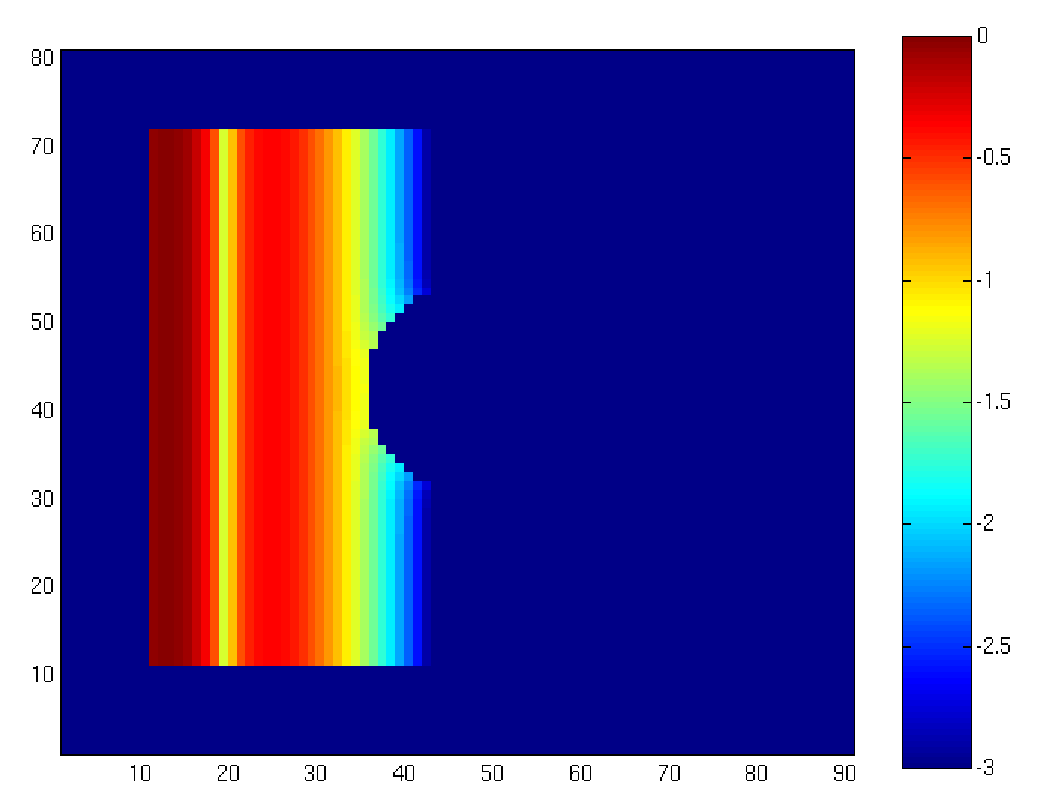
\epsfig{width=3in,file=Code/Fdtd-multidimensional/snapshot-sim6-te.eps}
  \\
  (a)
  \\
  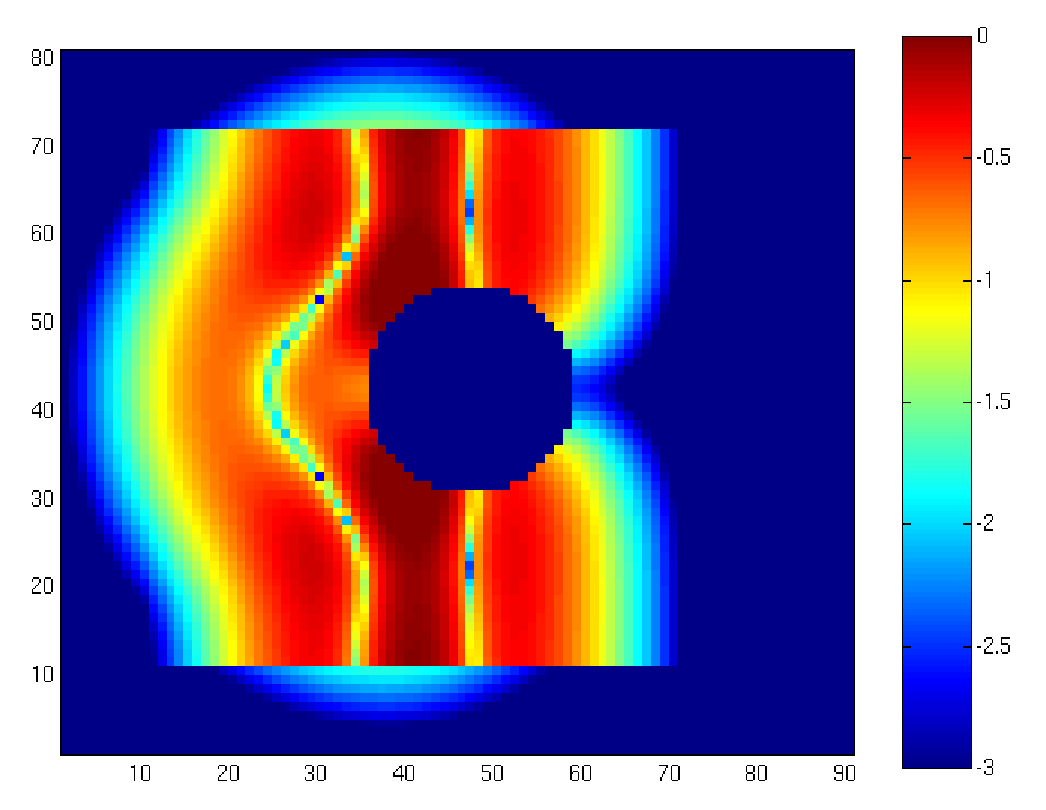
\epsfig{width=3in,file=Code/Fdtd-multidimensional/snapshot-sim10-te.eps}
  \\
  (b)
  \\
  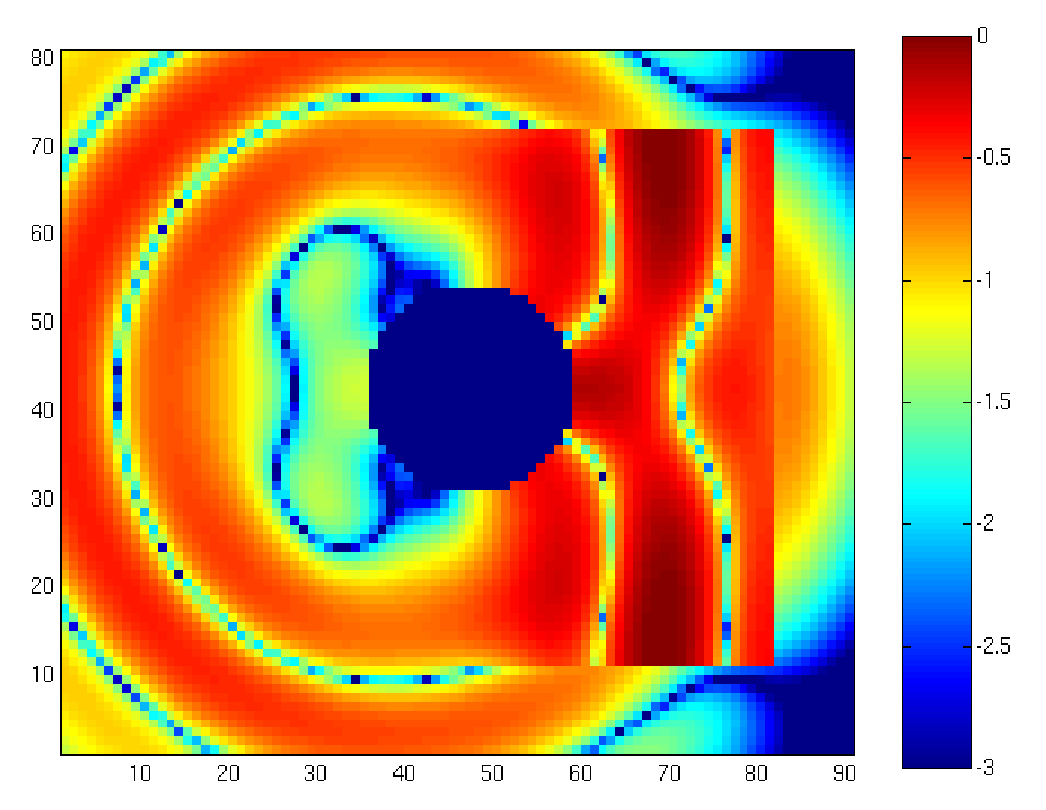
\epsfig{width=3in,file=Code/Fdtd-multidimensional/snapshot-sim14-te.eps}
  \\
  (c)
  \end{center} \caption{Pulsed TE$^z$ illumination of a circular
  scatter.  Display of the $H_z$ field at time-steps (a) $60$, (b)
  $100$ and (c) $140$.  The field has been normalized by $1/377$
  (i.e., the characteristic impedance of free space) and is shown with
  three decades of logarithmic scaling.  The incident field is a
  Ricker wavelet discretized such that there are $30$ points per
  wavelength at the most energetic frequency.}
  \label{fig:teScatterer}
\end{figure}
